%!TEX root = ../thesis.tex
%*******************************************************************************
%****************************** Second Chapter *********************************
%*******************************************************************************

\chapter{Score-based pullback Riemannian geometry}

\ifpdf
    \graphicspath{{Chapter5/Figs/Raster/}{Chapter5/Figs/PDF/}{Chapter5/Figs/}}
\else
    \graphicspath{{Chapter5/Figs/Vector/}{Chapter5/Figs/}}
\fi

Data-driven Riemannian geometry has emerged as a powerful tool for interpretable representation learning, offering improved efficiency in downstream tasks. Moving forward, it is crucial to balance cheap manifold mappings with efficient training algorithms. In this work, we integrate concepts from pullback Riemannian geometry and generative models to propose a framework for data-driven Riemannian geometry that is scalable in both geometry and learning: score-based pullback Riemannian geometry. Focusing on unimodal distributions as a first step, we propose a score-based Riemannian structure with closed-form geodesics that pass through the data probability density. With this structure, we construct a Riemannian autoencoder (RAE) with error bounds for discovering the correct data manifold dimension. This framework can naturally be used with anisotropic normalizing flows by adopting isometry regularization during training. Through numerical experiments on various datasets, we demonstrate that our framework not only produces high-quality geodesics through the data support, but also reliably estimates the intrinsic dimension of the data manifold and provides a global chart of the manifold, even in high-dimensional ambient spaces.

\section{Introduction}

Data often reside near low-dimensional non-linear manifolds as illustrated in \ref{fig:learned_charts}. This manifold assumption \cite{fefferman2016testing} has been popular since the early work on non-linear dimension reduction \cite{belkin2001laplacian,coifman2006diffusion,roweis2000nonlinear,sammon1969nonlinear,tenenbaum2000global}. Learning this non-linear structure, or representation learning, from data has proven to be highly successful \cite{demers1992non,kingma2013auto} and continues to be a recurring theme in modern machine learning approaches and downstream applications \cite{chow2022predicting,gomari2022variational,ternes2022multi,vahdat2020nvae,zhong2021cryodrgn}. 

Recent advances in data-driven Riemannian geometry have demonstrated its suitability for learning representations.
In this context, these representations are elements residing in a learned geodesic subspace of the data space, governed by a non-trivial Riemannian structure\footnote{rather than the standard $\ell^2$-inner product} across the entire ambient space \cite{arvanitidis2016locally,diepeveen2024pulling,hauberg2012geometric,peltonen2004improved,Scarvelis2023,sorrenson2024learningdistancesdatanormalizing,sun2024geometryaware}. 
Among these contributions, it is worth highlighting that \cite{sorrenson2024learningdistancesdatanormalizing} are the first and only ones so far to use information from the full data distribution obtained though generative models \cite{dinh2017density,song2020score}, even though this seems a natural approach given recent studies such as \cite{sakamoto2024the,stanczuk2022your}. A possible explanation for the limited use of generative models in constructing Riemannian geometry could lie in challenges regarding \emph{scalability of the manifold mappings}. Indeed, even though the generative models can be trained efficiently, \cite{sorrenson2024learningdistancesdatanormalizing} also mention themselves that it can be numerically challenging to work with their induced Riemannian geometry.

\begin{figure}[t]
    \centering
    \begin{subfigure}[b]{0.32\textwidth}
        \centering
        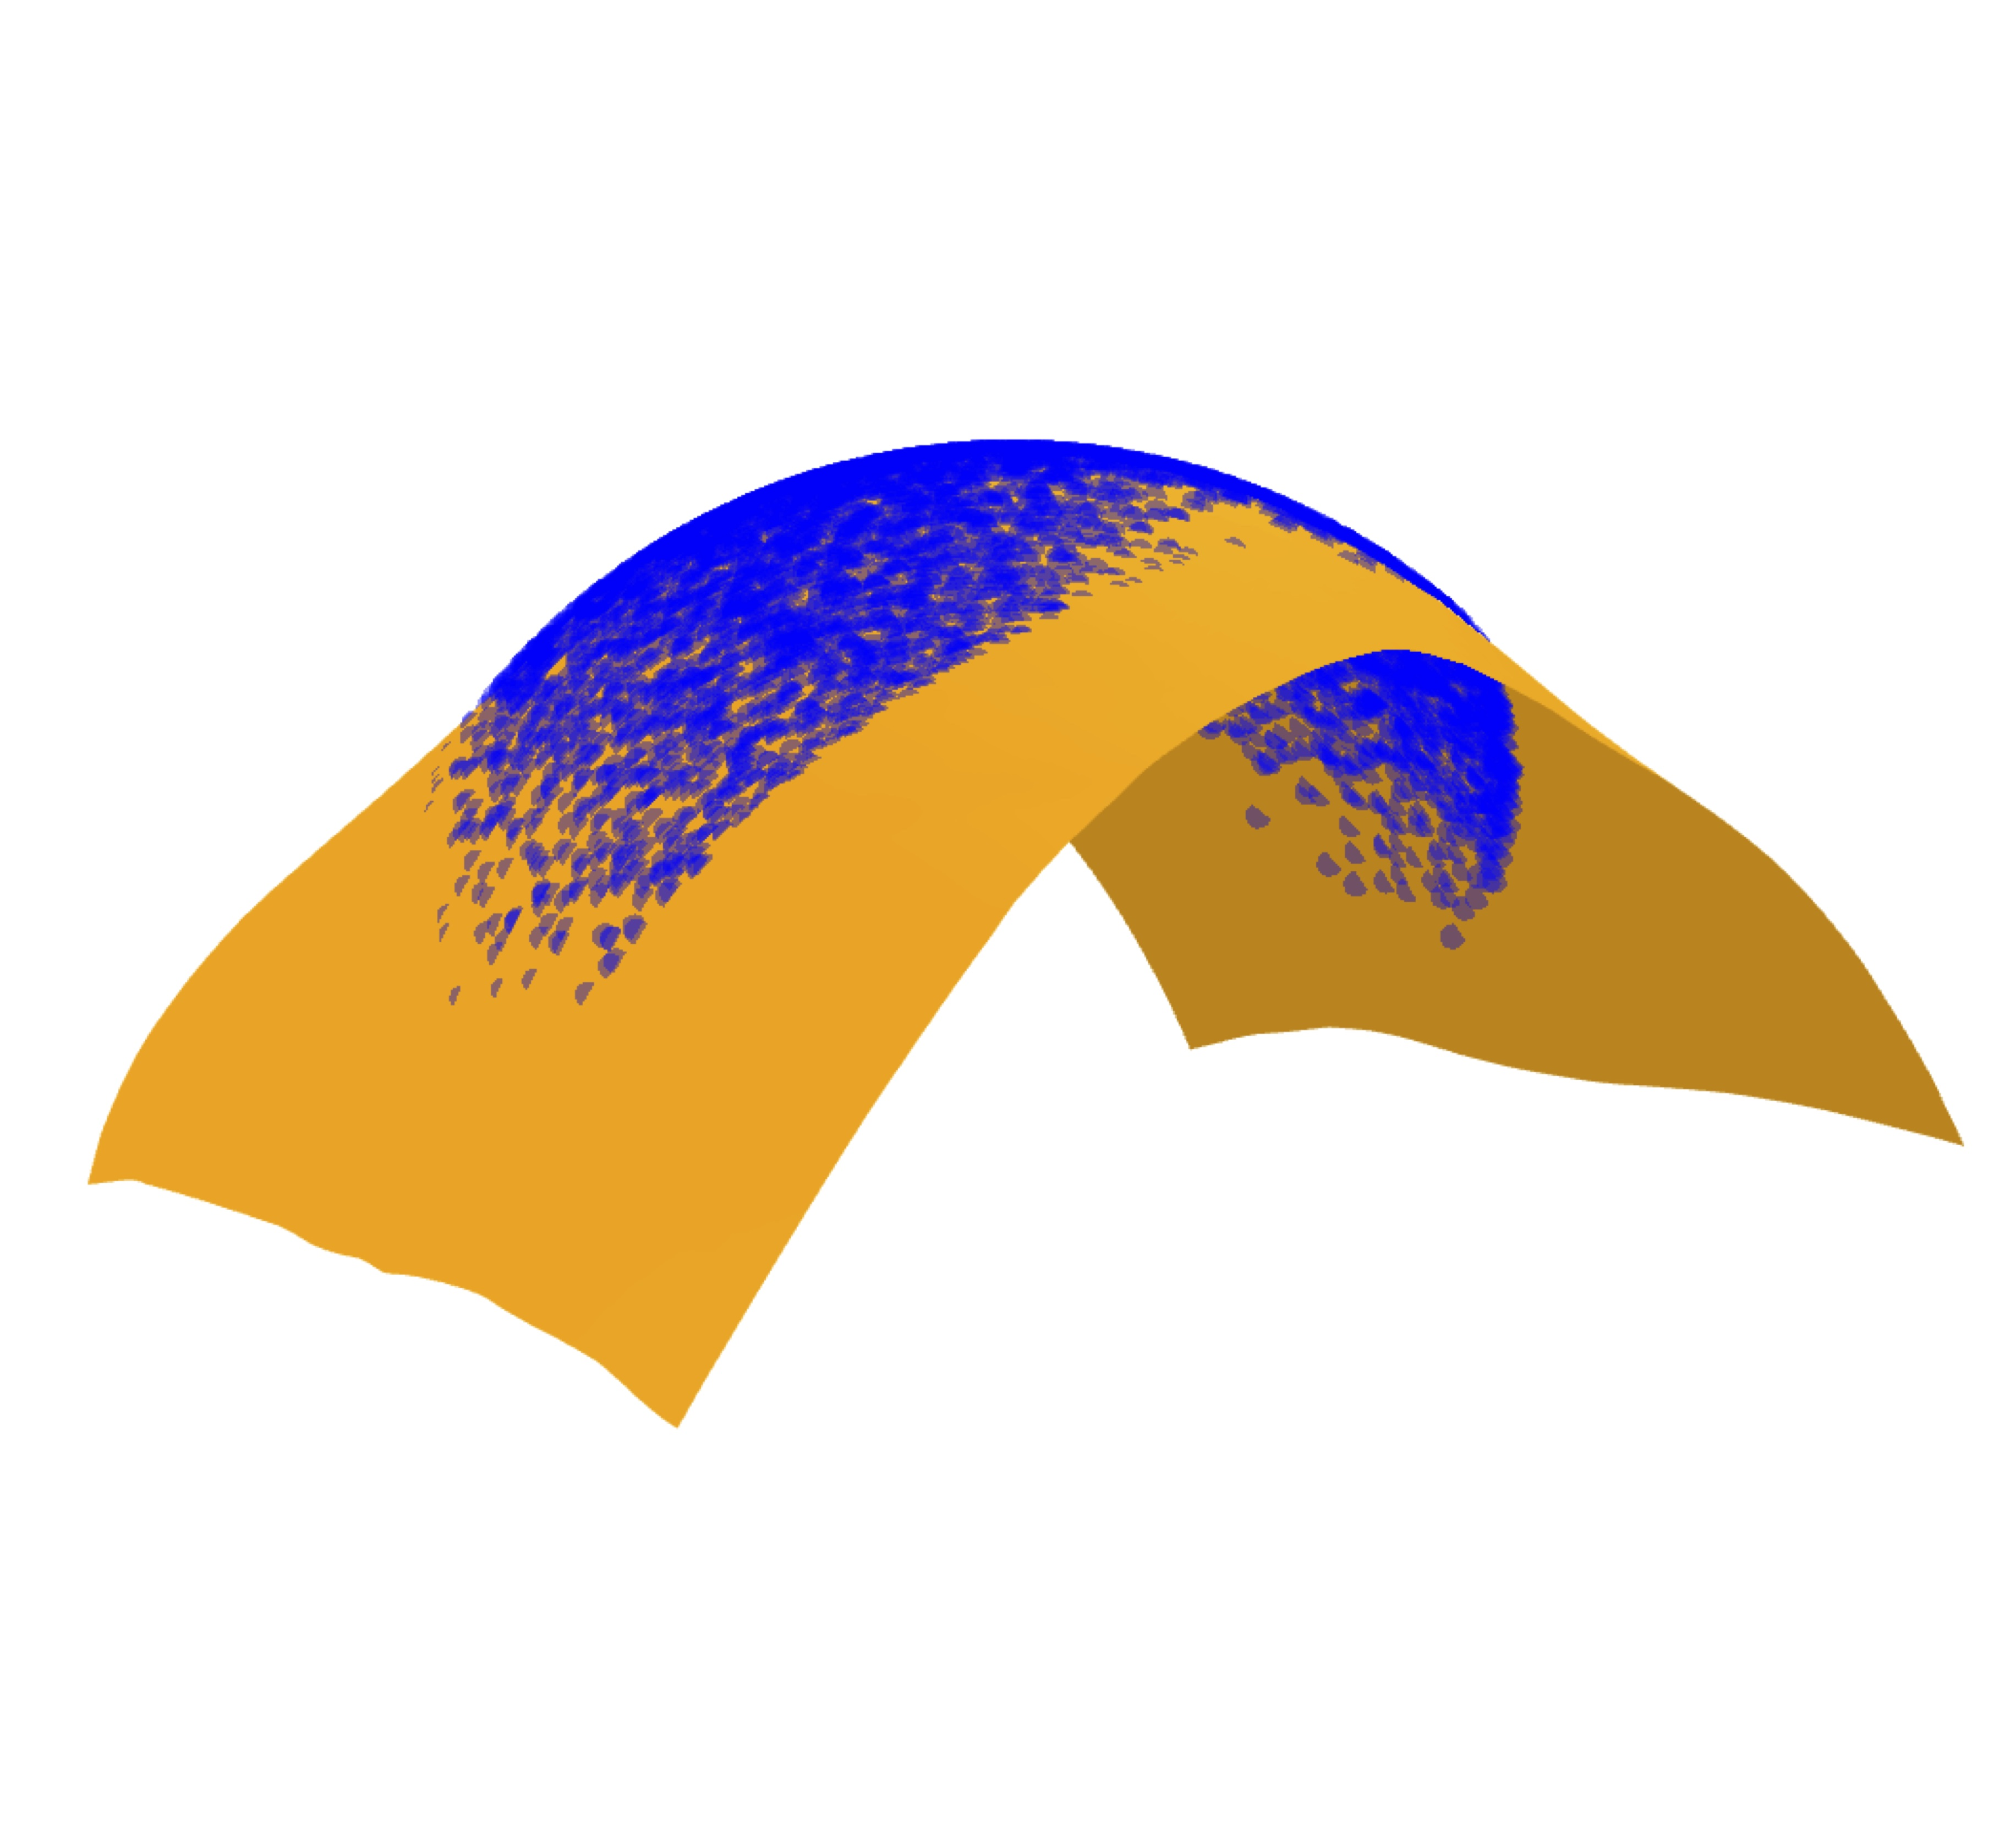
\includegraphics[width=\textwidth]{Chapter5/results/visualisations/RAE/projections/hemisphere_2_3/riemannian_autoencoder.jpg}
        \caption{Hemisphere (2,3)}
    \end{subfigure}
    \hfill
    \begin{subfigure}[b]{0.32\textwidth}
        \centering
        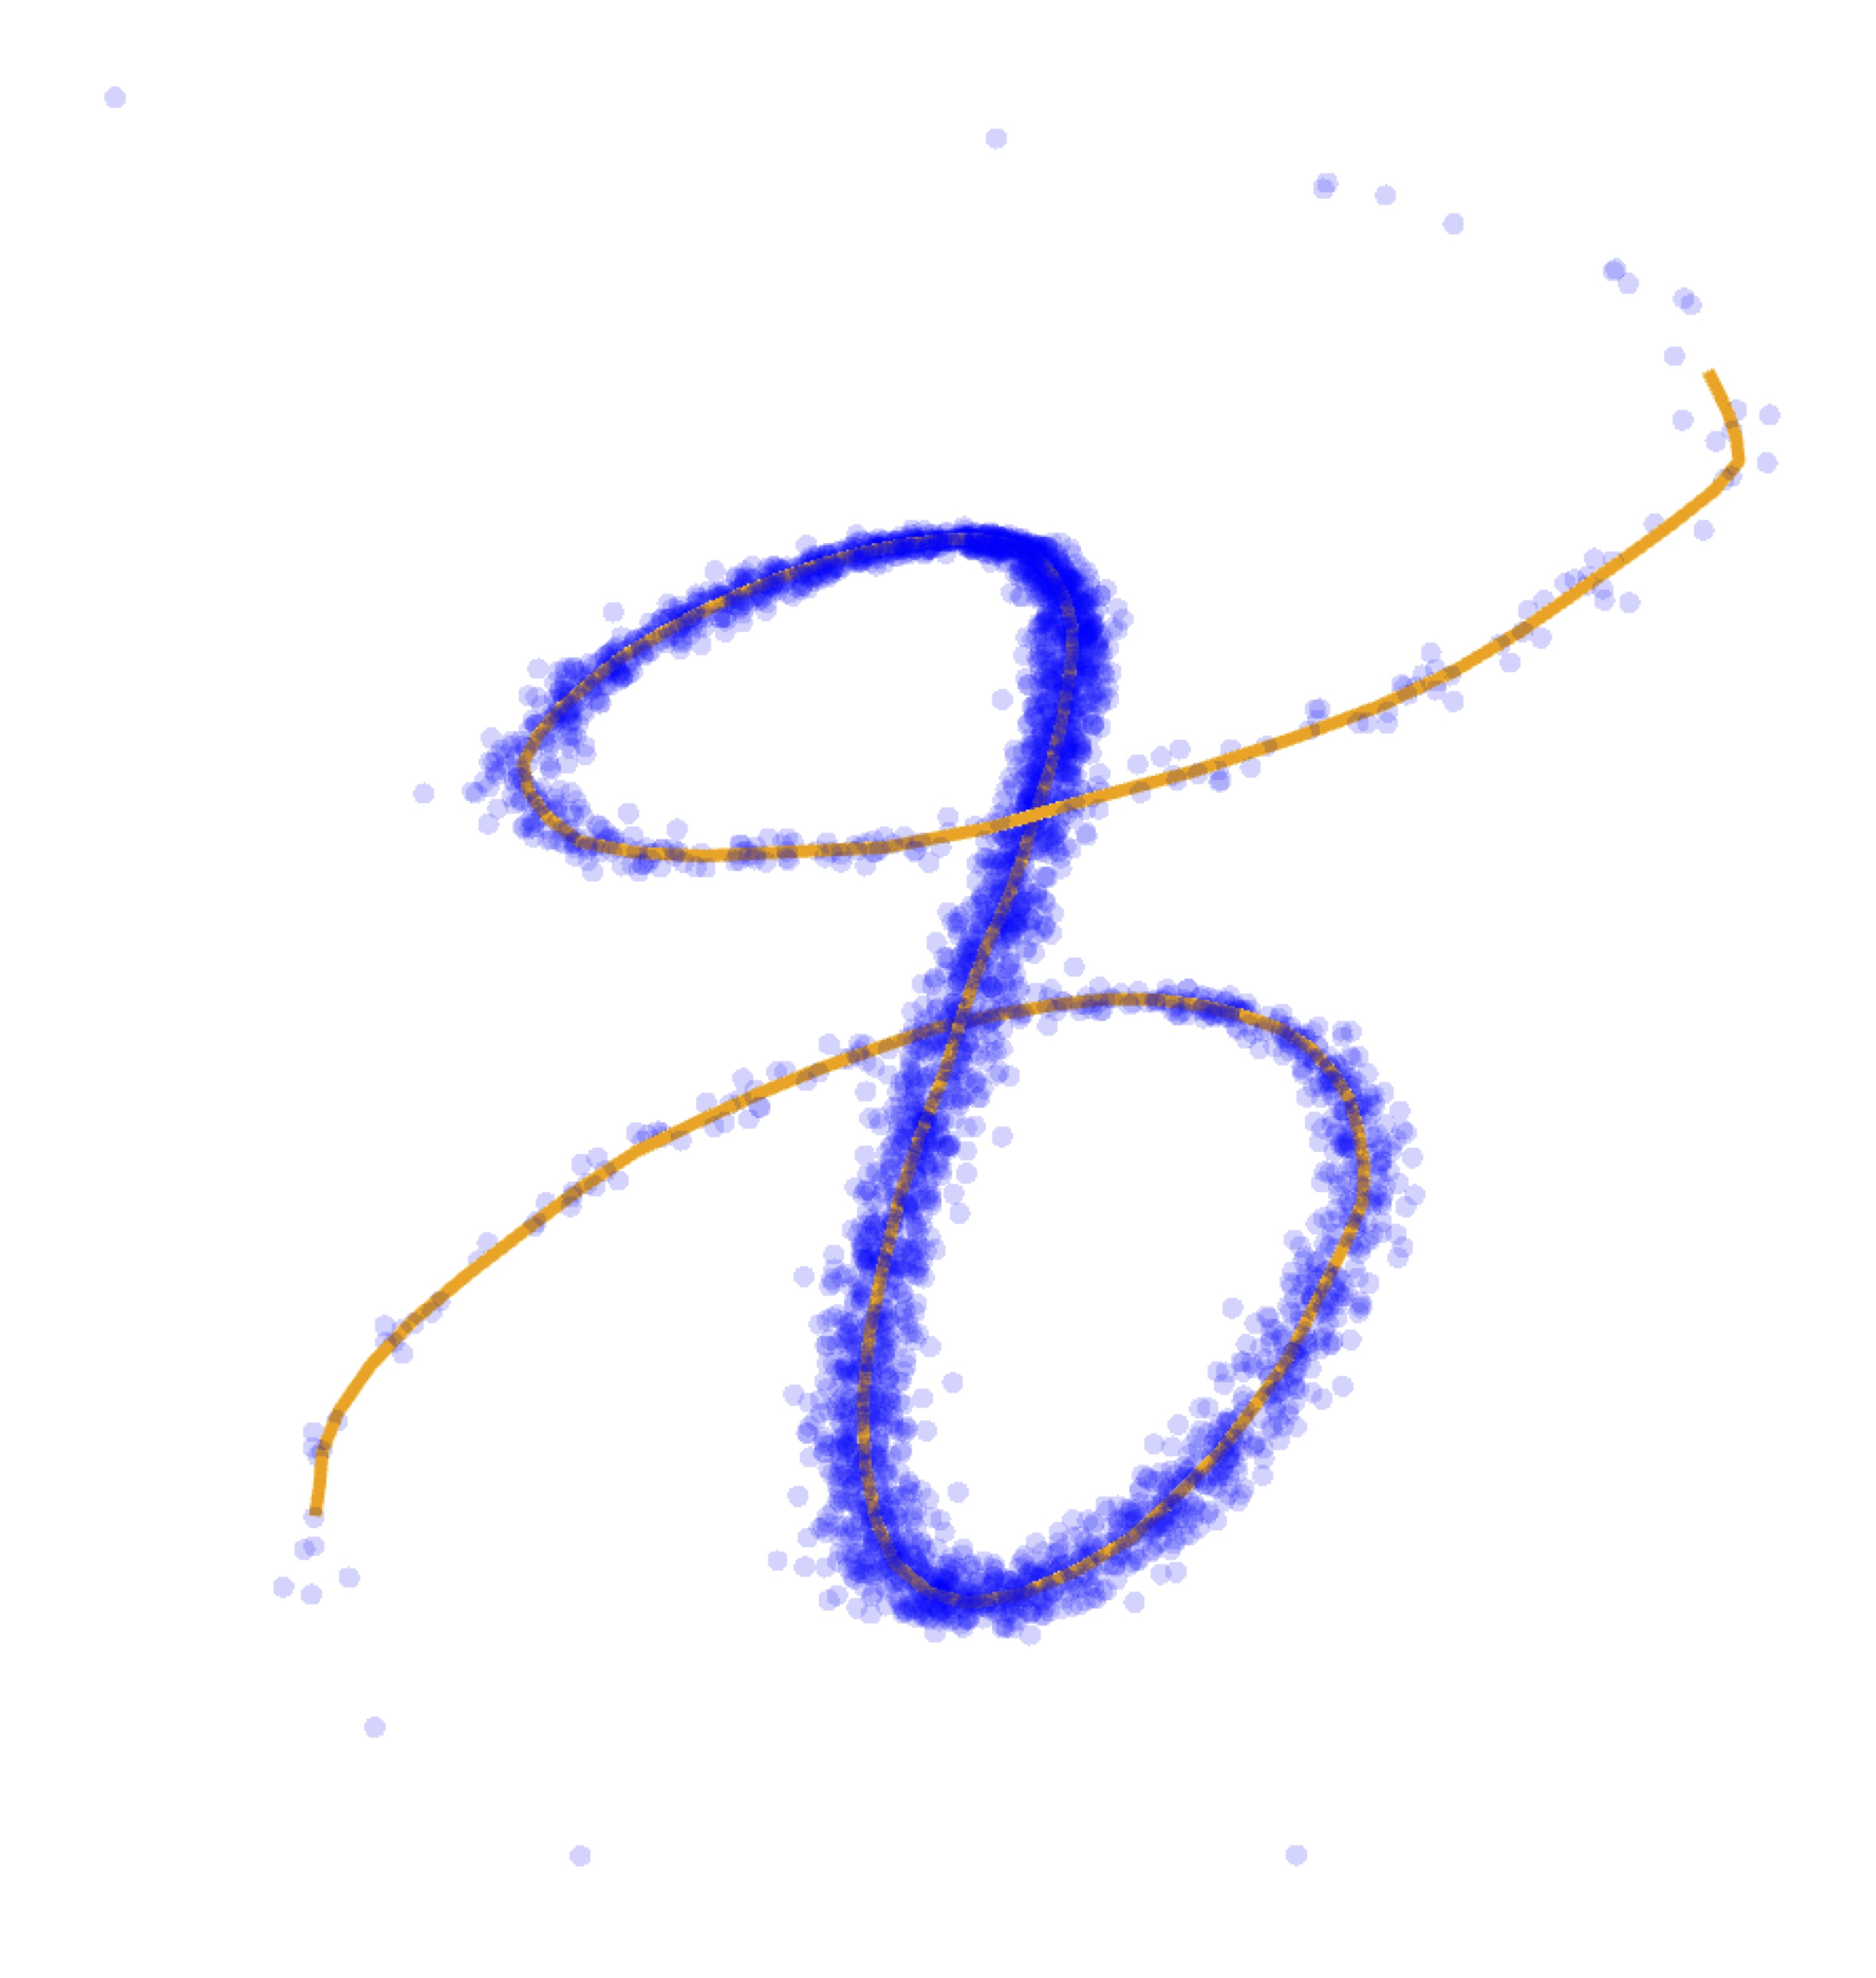
\includegraphics[width=\textwidth]{Chapter5/results/visualisations/RAE/projections/sinusoid_1_3/riemannian_autoencoder.jpg}
        \caption{Sinusoid (1,3)}
    \end{subfigure}
    \hfill
    \begin{subfigure}[b]{0.32\textwidth}
        \centering
        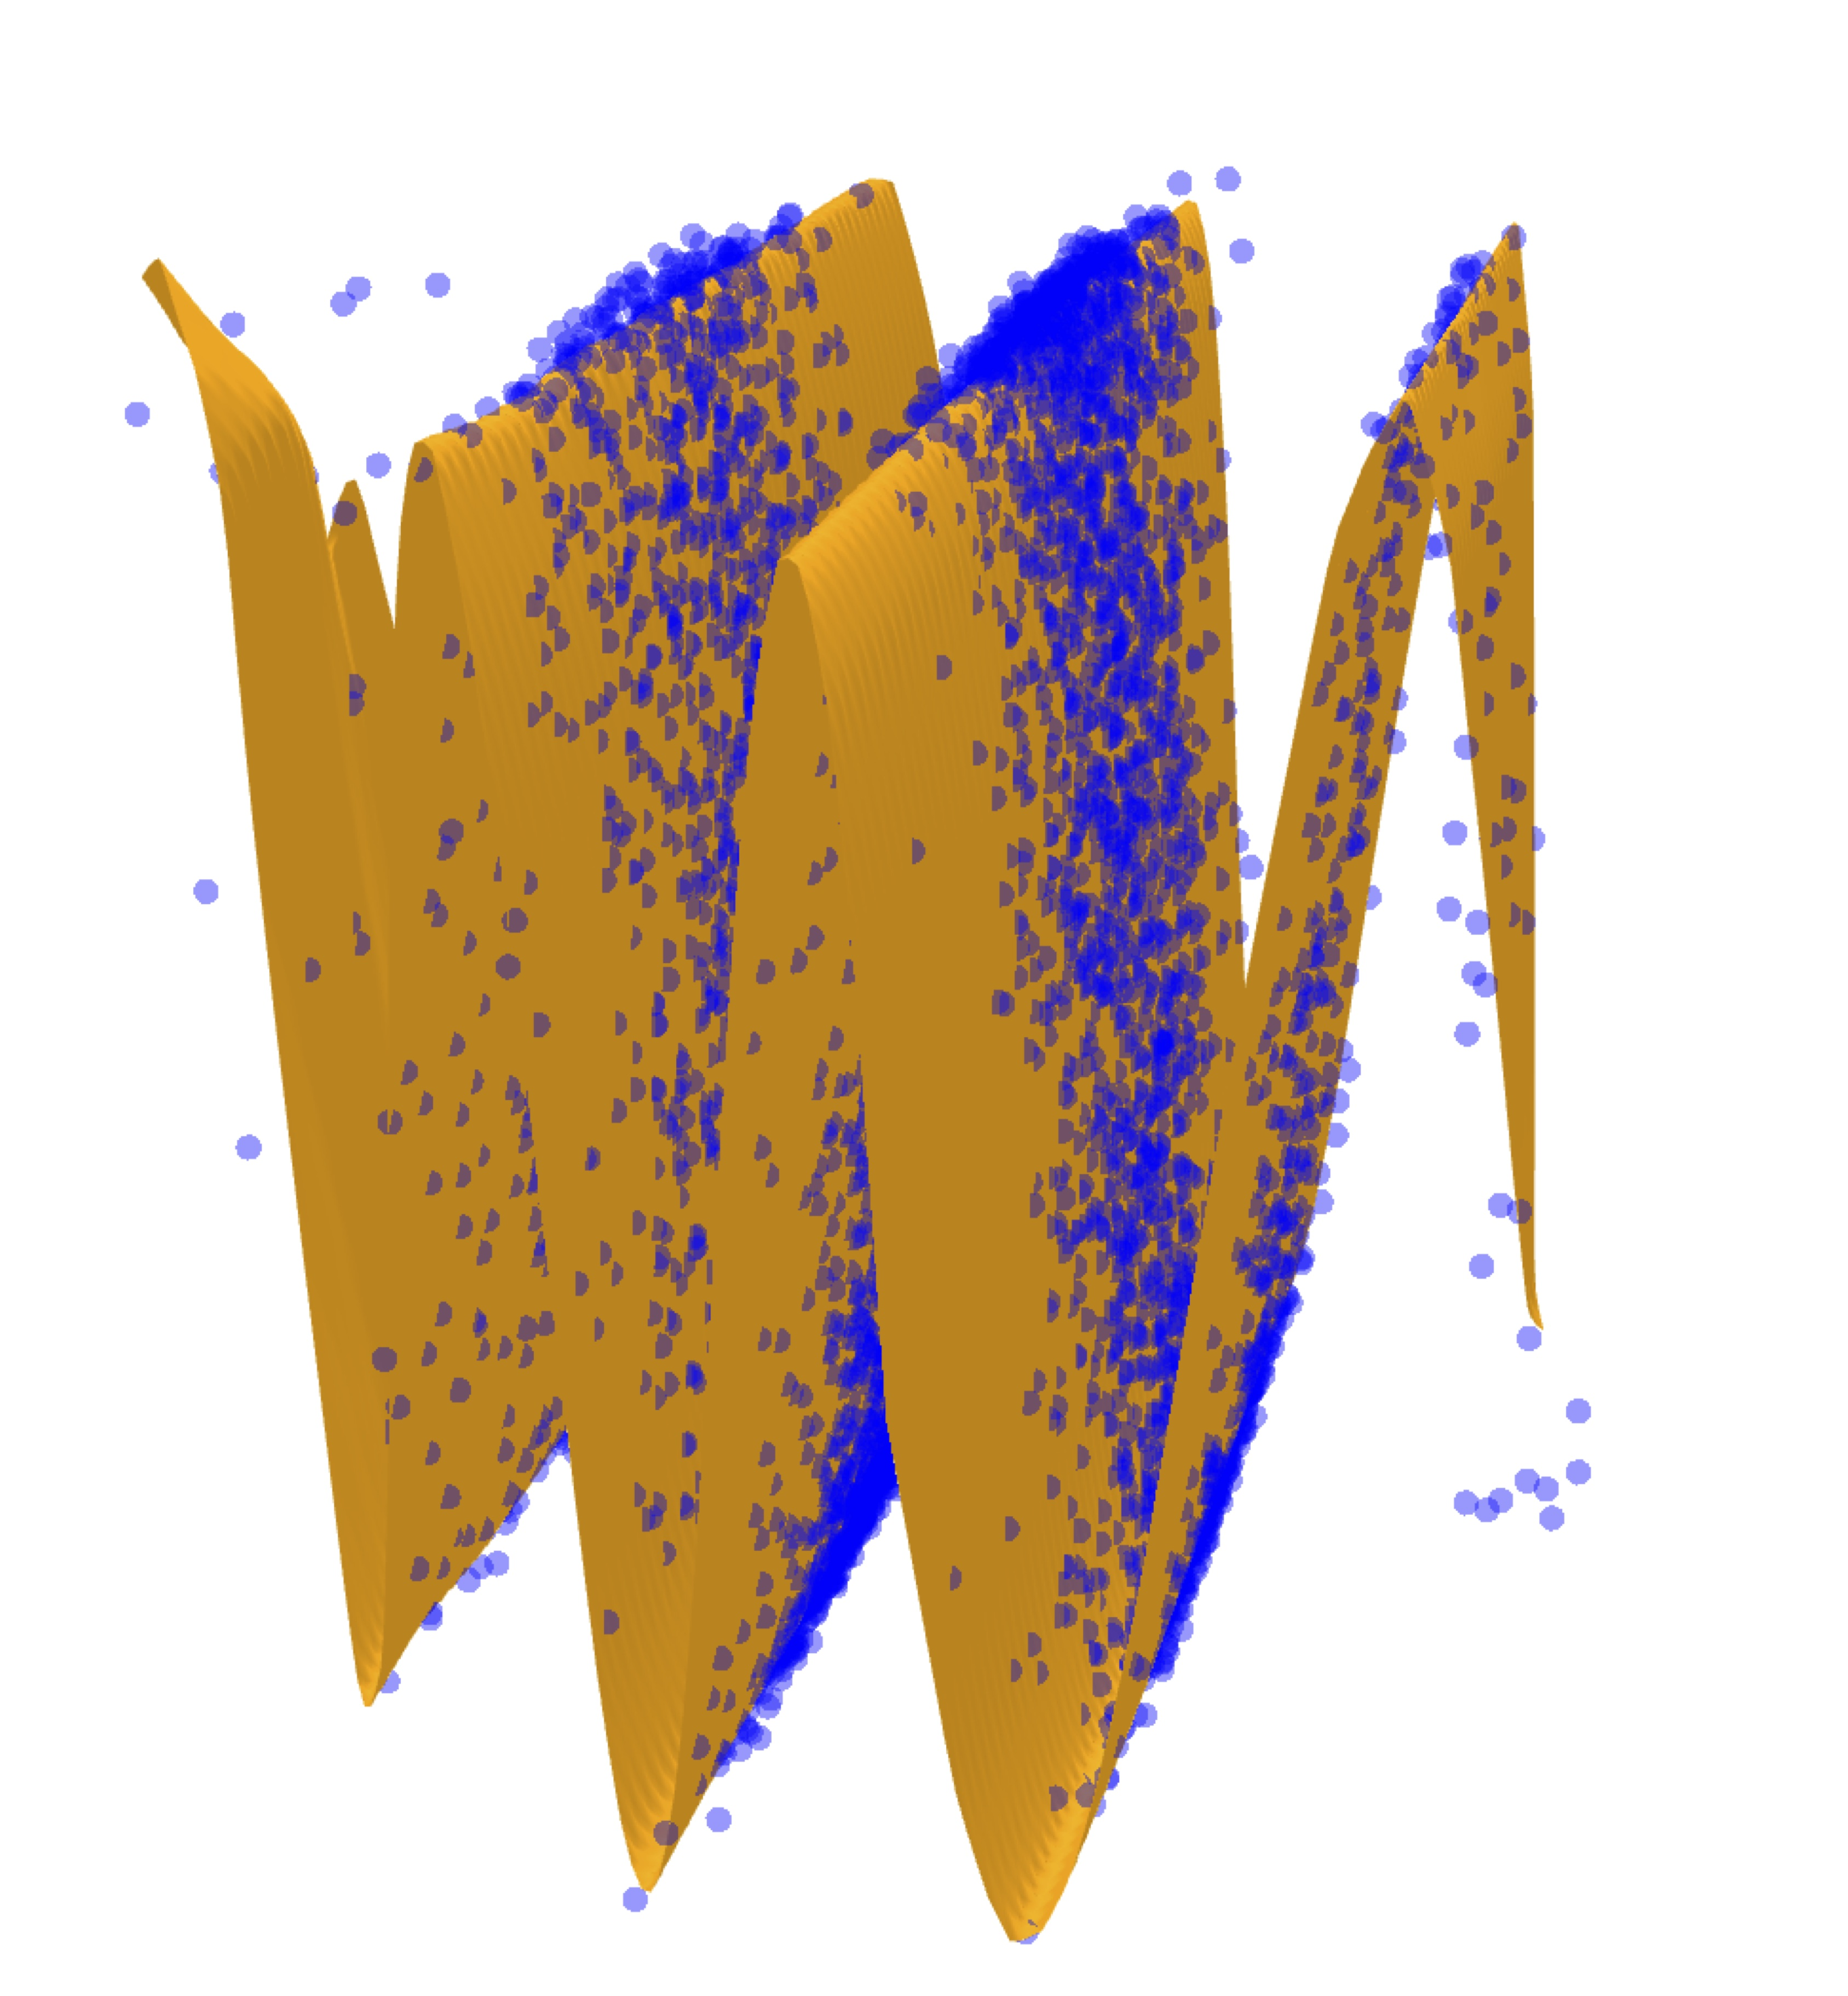
\includegraphics[width=\textwidth]{Chapter5/results/visualisations/RAE/projections/sinusoid_2_3/riemannian_autoencoder.jpg}
        \caption{Sinusoid (2,3)}
    \end{subfigure}

    \caption{
        Approximate data manifolds learned by the Riemannian autoencoder generated by score-based pullback Riemannian geometry for three datasets. The orange surfaces represent the manifolds learned by the model, while the blue points correspond to the training data. Each manifold provides a convincing low-dimensional representation of the data, isometric to its respective latent space.
    }
    \label{fig:learned_charts}
\end{figure}

If the manifold mapping scalability challenges were to be overcome, the combined power of Riemannian geometry and state of the art generative modelling could have profound implications on how to handle data in general. 
Indeed, beyond typical data analysis tasks such as computing distances, means, and interpolations/extrapolations of data points as illustrated in \ref{fig:toy-example}, a data-driven Riemannian structure also offers greater potential for representation learning and downstream applications. For instance, many advanced data processing methods, from Principal Component Analysis (PCA) to score and flow-matching, have Riemannian counterparts (\cite{diepeveen2023curvature,fletcher2004principal} and \cite{chen2023riemannian,huang2022riemannian}) that have proven beneficial by improving upon full black box methods in terms of interpretability \cite{diepeveen2024pulling} or Euclidean counterparts in terms of efficiency \cite{kapusniak2024metricflowmatchingsmooth}. 
 
Here it is worth highlighting that scalability of manifold mappings was completely circumvented by \cite{diepeveen2024pulling} by using pullback geometry. 
However, here learning a suitable (and stable) pullback geometry suffers from challenges regarding \emph{scalability of the training algorithm}, contrary to the approach by \cite{sorrenson2024learningdistancesdatanormalizing}.

Motivated by the above, this work aims to address the following question: How to strike a good balance between scalability of training a data-driven Riemannian structure and of evaluating its corresponding manifold mappings?

\begin{figure}[h!]
    \centering
    \begin{subfigure}{0.24\linewidth}
        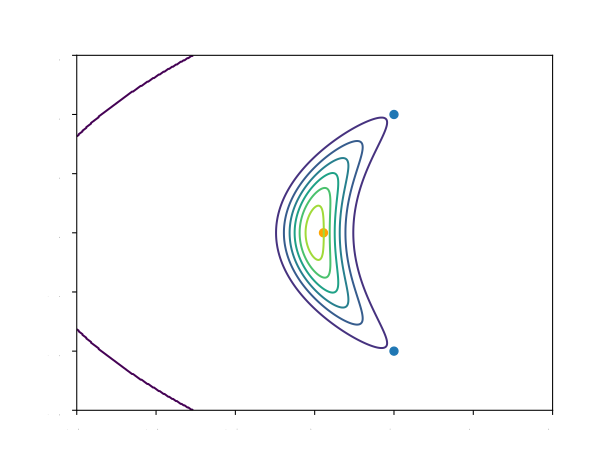
\includegraphics[width=\linewidth]{Chapter5/results/banana-distribution/barycentre.png}
        \caption{{Barycentre}}
        \label{fig:toy-example-barycentre}
    \end{subfigure}
    \begin{subfigure}{0.24\linewidth}
        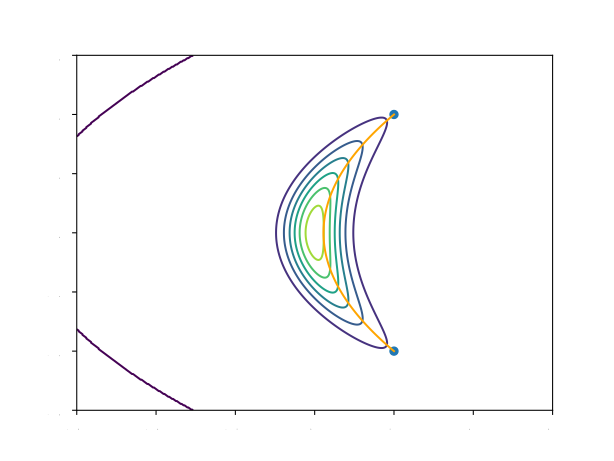
\includegraphics[width=\linewidth]{Chapter5/results/banana-distribution/geodesic.png}
        \caption{{Geodesic}}
        \label{fig:toy-example-geodesic}
    \end{subfigure}
    \begin{subfigure}{0.24\linewidth}
        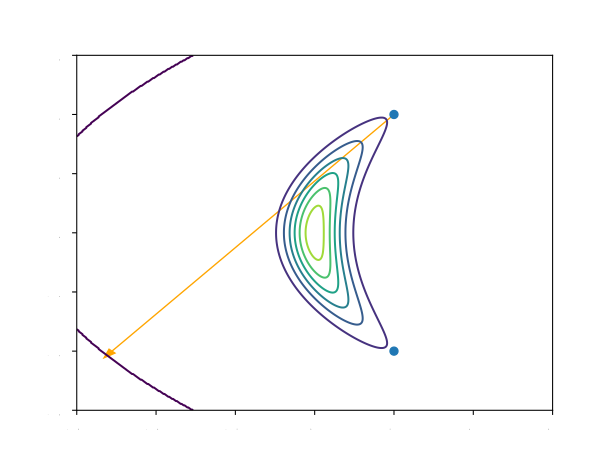
\includegraphics[width=\linewidth]{Chapter5/results/banana-distribution/logarithmic.png}
        \caption{{Logarithm}}
        \label{fig:toy-example-log}
    \end{subfigure}
    \begin{subfigure}{0.24\linewidth}
        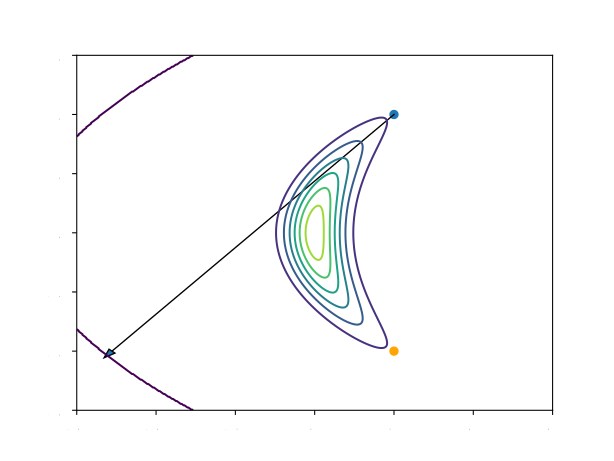
\includegraphics[width=\linewidth]{Chapter5/results/banana-distribution/exponential.png}
        \caption{{Exponential}}
        \label{fig:toy-example-exp}
    \end{subfigure}
    \caption{Score-based pullback Riemannian geometry (proposed) from a toy probability density.}
    \label{fig:toy-example}
\end{figure}

\subsection{Contributions}

In this paper, we take first steps towards striking such a balance and propose a score-based pullback Riemannian metric assuming a relatively simple but generally applicable family of probability densities, which we show to result in both scalable manifold mappings and scalable learning algorithms. We emphasize that we do not directly aim to find the perfect balance between the two types of scalability. Instead we start from a setting which has many nice properties, but will allow for generalization to multimodal densities, which we reserve for future work.

Specifically, we consider a family of unimodal probability densities whose negative log-likelihoods are compositions of strongly convex functions and diffeomorphisms. As this work is an attempt to bridge between the geometric data analysis community and the generative modeling community, we break down the contributions in two ways.
Theoretically,
\begin{itemize}
    \item We propose a score-based pullback Riemannian metric such that manifold mappings respect the data distribution as illustrated in \ref{fig:toy-example-barycentre},\ref{fig:toy-example-geodesic},\ref{fig:toy-example-log},\ref{fig:toy-example-exp}.
    \item We demonstrate that this density-based Riemannian structure naturally leads to a Riemannian autoencoder\footnote{in the sense of \cite{diepeveen2024pulling}} and provide error bounds on the expected reconstruction error, which allows for approximation of the data manifold as illustrated in \ref{fig:learned_charts}.
    \item We introduce a learning scheme based on adaptations of normalizing flows to find the density to be integrated into the Riemannian framework, which is tested on several synthetic data sets. 
\end{itemize}
Practically, this work showcases how two simple adaptations to the normalizing flows framework enable data-driven Riemannian geometry. This significantly expands the potential for downstream applications compared to the unadapted framework.

\subsection{Outline}

After introducing notation in \ref{sec:notation}, \ref{sec:unimodal-riemannian geometry} considers a family of probability distributions, from which we obtain suitable geometry, and \ref{sec:rae} showcases how one can subsequently construct Riemannian Autoencoders with theoretical guarantees. From these observations \ref{sec:adapting-normalizing-flows} discusses the natural limitations of standard normalizing flows and how to change the parametrisation and training for downstream application in a Riemannian geometric setting. \ref{sec:numerics} showcases several use cases of data-driven Riemannian structure on several data sets. Finally, we summarize our findings in \ref{sec:conclusions}.

\section{Notation}
\label{sec:notation}

Here we present some basic notations from differential and Riemannian geometry, see \cite{boothby2003introduction,carmo1992riemannian,lee2013smooth,sakai1996riemannian} for details. 

Let $\manifold$ be a smooth manifold. We write $C^\infty(\manifold)$ for the space of smooth functions over $\manifold$. The \emph{tangent space} at $\mPoint \in \manifold$, which is defined as the space of all \emph{derivations} at $\mPoint$, is denoted by $\tangent_\mPoint \manifold$ and for \emph{tangent vectors} we write $\tangentVector_\mPoint \in \tangent_\mPoint \manifold$. For the \emph{tangent bundle} we write $\tangent\manifold$ and smooth vector fields, which are defined as \emph{smooth sections} of the tangent bundle, are written as $\vectorfield(\manifold) \subset \tangent\manifold$.

A smooth manifold $\manifold$ becomes a \emph{Riemannian manifold} if it is equipped with a smoothly varying \emph{metric tensor field} $(\,\cdot\,, \,\cdot\,) \colon \vectorfield(\manifold) \times \vectorfield(\manifold) \to C^\infty(\manifold)$. This tensor field induces a \emph{(Riemannian) metric} $\distance_{\manifold} \colon \manifold\times\manifold\to\Real$. The metric tensor can also be used to construct a unique affine connection, the \emph{Levi-Civita connection}, that is denoted by $\nabla_{(\,\cdot\,)}(\,\cdot\,) : \vectorfield(\manifold) \times \vectorfield(\manifold) \to \vectorfield(\manifold)$. 
This connection is in turn the cornerstone of a myriad of manifold mappings.
One is the notion of a \emph{geodesic}, which for two points $\mPoint,\mPointB \in \manifold$ is defined as a curve $\geodesic_{\mPoint,\mPointB} \colon [0,1] \to \manifold$ with minimal length that connects $\mPoint$ with $\mPointB$. 
Another closely related notion to geodesics is the curve $t \mapsto \geodesic_{\mPoint,\tangentVector_\mPoint}(t)$  for a geodesic starting from $\mPoint\in\manifold$ with velocity $\dot{\geodesic}_{\mPoint,\tangentVector_\mPoint} (0) = \tangentVector_\mPoint \in \tangent_\mPoint\manifold$. This can be used to define the \emph{exponential map} $\exp_\mPoint \colon \mathcal{D}_\mPoint \to \manifold$ as 
\begin{equation}
\exp_\mPoint(\tangentVector_\mPoint) := \geodesic_{\mPoint,\tangentVector_\mPoint}(1)
\quad\text{where $\mathcal{D}_\mPoint \subset \tangent_\mPoint\manifold$ is the set on which $\geodesic_{\mPoint,\tangentVector_\mPoint}(1)$ is defined.} 
\end{equation}
Furthermore, the \emph{logarithmic map} $\log_\mPoint \colon \exp(\mathcal{D}'_\mPoint ) \to \mathcal{D}'_\mPoint$ is defined as the inverse of $\exp_\mPoint$, so it is well-defined on  $\mathcal{D}'_{\mPoint} \subset \mathcal{D}_{\mPoint}$ where $\exp_\mPoint$ is a diffeomorphism. 

Finally, if $(\manifold, (\cdot,\cdot))$ is a $\dimInd$-dimensional Riemannian manifold, $\manifoldB$ is a $\dimInd$-dimensional smooth manifold and $\diffeoB:\manifoldB \to \manifold$ is a diffeomorphism, the \emph{pullback metric}
\begin{equation}
    (\tangentVector, \tangentVectorB)^\diffeoB := (D_{(\cdot)}\diffeoB[\tangentVector_{(\cdot)}], D_{(\cdot)}\diffeoB[\tangentVectorB_{(\cdot)}])_{\diffeoB(\cdot)},
    \label{eq:pull-back-metric}
\end{equation}
where $D_{\mPoint}\diffeoB: \tangent_\mPoint \manifoldB \to \tangent_{\diffeoB(\mPoint)} \manifold$ denotes the differential of $\diffeoB$,

defines a Riemannian structure on $\manifoldB$, which we denote by $(\manifoldB, (\cdot,\cdot)^\diffeoB)$. 
Pullback metrics literally pull back all geometric information from the Riemannian structure on $\manifold$. In particular, closed-form manifold mappings on $(\manifold, (\cdot,\cdot))$ yield under mild assumptions closed-form manifold mappings on $(\manifoldB, (\cdot,\cdot)^\diffeoB)$.
Throughout the rest of the paper pullback mappings will be denoted similarly to \ref{eq:pull-back-metric} with the diffeomorphism $\diffeoB$ as a superscript, i.e., we write $\distance^\diffeoB_{\manifoldB}(\mPoint, \mPointB)$, $\geodesic^\diffeoB_{\mPoint, \mPointB}$, $\exp^\diffeoB_\mPoint (\tangentVector_\mPoint)$ and $\log^\diffeoB_{\mPoint} \mPointB$ 
for $\mPoint,\mPointB \in \manifoldB$ and $\tangentVector_\mPoint \in \tangent_\mPoint \manifoldB$. 

\section{Riemannian geometry from unimodal probability densities}
\label{sec:unimodal-riemannian geometry}

We remind the reader that the ultimate goal of data-driven Riemannian geometry on $\Real^\dimInd$ is to construct a Riemannian structure such that geodesics always pass through the support of data probability densities. In this section we will focus on constructing Riemannian geometry that does just that from unimodal densities $\density:\Real^\dimInd\to \Real$ of the form
\begin{equation}
    \density(\Vector) \propto e^{- \stroco(\diffeo(\Vector))}
    \label{eq:stroco-diffeo-density}
\end{equation}

where $\stroco:\Real^\dimInd\to\Real$ is a smooth strongly convex function and $\diffeo:\Real^\dimInd\to\Real^\dimInd$ is a diffeomorphism, e.g., such as the density in \ref{fig:toy-example}\footnote{Here, $\stroco(\Vector) := 2 \Vector_1^2 + \frac{1}{8}\Vector_2^2$ and $\diffeo(\Vector):= (\Vector_1 - \frac{1}{9} \Vector_2^2, \Vector_2)$.}. In particular, we will consider pullback Riemannian structures of the form
\begin{equation}
    (\tangentVector, \tangentVectorB)^{\nabla \stroco \circ \diffeo}_{\Vector} := (D_{\Vector} \nabla \stroco \circ \diffeo[\tangentVector], D_{\Vector} \nabla \stroco \circ \diffeo[\tangentVectorB])_2,
    \label{eq:stroco-diffeo-pullback}
\end{equation}
which are related to the Riemannian structure obtained from the \emph{score function} $\nabla \log(\density(\cdot)):\Real^\dimInd\to\Real^\dimInd$ if $\diffeo$ is close to a linear $\ell^2$-isometry on the data support, i.e., $D_{\Vector} \diffeo$ is an orthogonal operator:
\begin{multline}
    (D_{\Vector} \nabla \log(\density(\cdot))[\tangentVector], D_{\Vector} \nabla \log(\density(\cdot))[\tangentVectorB])_2 = (D_{\Vector} \nabla (\stroco \circ \diffeo)[\tangentVector], D_{\Vector} \nabla (\stroco \circ \diffeo)[\tangentVectorB])_2 \\
    = (D_{\Vector} ((D_{(\cdot)} \diffeo)^{\top} \circ \nabla\stroco \circ \diffeo)[\tangentVector], D_{\Vector}((D_{(\cdot)} \diffeo)^{\top} \circ \nabla\stroco \circ \diffeo) [\tangentVectorB])_2 \\
    \approx (D_{\Vector} \nabla \stroco \circ \diffeo[\tangentVector], D_{\Vector} \nabla \stroco \circ \diffeo[\tangentVectorB])_2 = (\tangentVector, \tangentVectorB)^{\nabla \stroco \circ \diffeo}_{\Vector}.
\end{multline}
For that reason, we call such an approach to data-driven Riemannian geometry: \emph{score-based pullback Riemannian geometry}. Since we find ourselves in a pullback setting\footnote{This is generally not true when using the score itself for probability densities of the form \ref{eq:stroco-diffeo-density}.}, this allows to construct pullback geometry with closed-form manifold mappings.

What remains to be shown is that such geodesics and other manifold mappings pass through the data support (like in \ref{fig:toy-example-barycentre},\ref{fig:toy-example-geodesic},\ref{fig:toy-example-log},\ref{fig:toy-example-exp}). 

The following result, which is a direct application of \cite[Prop.~2.1]{diepeveen2024pulling} and \cite[Cor.~3.6.1]{diepeveen2024pulling}, gives us closed-form expressions of several important manifold mappings under $(\cdot,\cdot)^{\nabla \stroco \circ \diffeo}$ and makes a connection with $(\cdot,\cdot)^{\diffeo}$ if we choose
\begin{equation}
    \stroco(\Vector)=\frac{1}{2} \Vector^{\top} \spdMatrix^{-1} \Vector,
    \label{eq:quadratic-stroco}
\end{equation}
where $\spdMatrix\in \Real^{\dimInd\times \dimInd}$ is symmetric positive definite. 

This special case highlights why, in general, we obtain geodesics and manifold mappings that pass through the data support. For instance, in the scenario depicted in \ref{fig:toy-example-geodesic}, where the correct form \ref{eq:stroco-diffeo-density} is used, geodesics are computed by first reversing the effect of the diffeomorphism -- transforming the data distribution to resemble a Gaussian, then drawing straight lines between the morphed data points, and finally applying the diffeomorphism again. This approach results in geodesics that traverse regions of higher likelihood between the endpoints, due to the strong convexity of the quadratic function, which aligns perfectly with our objectives.

\begin{proposition}
    \label{thm:pull-back-mappings}
        Let $\diffeo:\Real^\dimInd \to \Real^\dimInd$ be a smooth diffeomorphism and let $\stroco: \Real^\dimInd \to \Real$ be a smooth strongly convex function, whose Fenchel conjugate is denoted by $\stroco^\star: \Real^\dimInd\to\Real$. Next, consider the $\ell^2$-pullback manifolds $(\Real^\dimInd, (\cdot,\cdot)^{\nabla \stroco \circ \diffeo})$ and $(\Real^\dimInd, (\cdot,\cdot)^{\diffeo})$ defined through metric tensor fields
        \begin{equation}
            (\tangentVector, \tangentVectorB)^{\nabla \stroco \circ \diffeo}_{\Vector} := (D_{\Vector} \nabla \stroco \circ \diffeo[\tangentVector], D_{\Vector} \nabla \stroco \circ \diffeo[\tangentVectorB])_2, \quad \text{and} \quad (\tangentVector, \tangentVectorB)^{\diffeo}_{\Vector} := (D_{\Vector} \diffeo[\tangentVector], D_{\Vector} \diffeo[\tangentVectorB])_2.
        \end{equation}
    
        Then,
        \begin{enumerate}[label=(\roman*)]
            \item length-minimising geodesics $\geodesic^{\nabla \stroco \circ \diffeo}_{\Vector, \VectorB}:[0,1] \to \Real^\dimInd$ on $(\Real^\dimInd, (\cdot,\cdot)^{\nabla \stroco \circ \diffeo})$ are given by 
            \begin{equation}
                \geodesic^{\nabla \stroco \circ \diffeo}_{\Vector, \VectorB}(t)= (\diffeo^{-1} \circ\nabla \stroco^*) ((1 - t)(\nabla \stroco \circ \diffeo)(\Vector) + t (\nabla \stroco \circ \diffeo)(\VectorB)).
                \label{eq:thm-geodesic-remetrized}
            \end{equation}
            In addition, if $\stroco$ is of the form \ref{eq:quadratic-stroco}
            \begin{equation}
                \geodesic^{\nabla \stroco \circ \diffeo}_{\Vector, \VectorB}(t) = \geodesic^\diffeo_{\Vector, \VectorB}(t) = \diffeo^{-1}((1 - t)\diffeo(\Vector) + t \diffeo(\VectorB)).
                \label{eq:thm-geodesic-remetrized-special-psi}
            \end{equation}
            \item the logarithmic map $\log^{\nabla \stroco \circ \diffeo}_{\Vector} (\cdot):\Real^\dimInd \to \tangent_\Vector \Real^\dimInd$  on $(\Real^\dimInd, (\cdot,\cdot)^{\nabla \stroco \circ \diffeo})$ is given by 
            \begin{equation}
                \log^{\nabla \stroco \circ \diffeo}_{\Vector} \VectorB =  D_{\diffeo(\Vector)}\diffeo^{-1}[D_{(\nabla \stroco \circ \diffeo)(\Vector)}\nabla \stroco^*[(\nabla \stroco \circ \diffeo)(\VectorB) - (\nabla \stroco \circ \diffeo)(\Vector)]].
                \label{eq:thm-log-remetrized}
            \end{equation}
            In addition, if $\stroco$ is of the form \ref{eq:quadratic-stroco}
            \begin{equation}
                \log^{\nabla \stroco \circ \diffeo}_{\Vector} \VectorB = \log^\diffeo_{\Vector} \VectorB = D_{\diffeo(\Vector)}\diffeo^{-1}[\diffeo(\VectorB) - \diffeo(\Vector)].
                \label{eq:thm-log-remetrized-special-psi}
            \end{equation}
            \item the exponential map $\exp^{\nabla \stroco \circ \diffeo}_{\Vector} (\cdot):\tangent_\Vector \Real^\dimInd \to \Real^\dimInd$ on $(\Real^\dimInd, (\cdot,\cdot)^{\nabla \stroco \circ \diffeo})$ is given by 
            \begin{equation}
                 \exp^{\nabla \stroco \circ \diffeo}_\Vector (\tangentVector_\Vector) = (\diffeo^{-1} \circ\nabla \stroco^*)((\nabla \stroco \circ \diffeo)(\Vector) + D_{\diffeo(\Vector)} \nabla \stroco [ D_{\Vector} \diffeo[\tangentVector_\Vector] ]).
                 \label{eq:thm-exp-remetrized}
            \end{equation}
            In addition, if $\stroco$ is of the form \ref{eq:quadratic-stroco}
            \begin{equation}
                 \exp^{\nabla \stroco \circ \diffeo}_\Vector (\tangentVector_\Vector) = \exp^\diffeo_\Vector (\tangentVector_\Vector) = \diffeo^{-1}(\diffeo(\Vector) + D_{\Vector} \diffeo[\tangentVector_\Vector]).
                 \label{eq:thm-exp-remetrized-special-psi}
            \end{equation}
            \item the distance $\distance^{\nabla \stroco \circ \diffeo}_{\Real^\dimInd}:\Real^\dimInd \times\Real^\dimInd \to \Real$ on $(\Real^\dimInd, (\cdot,\cdot)^{\nabla \stroco \circ \diffeo})$ is given by 
            \begin{equation}
                \distance^{\nabla \stroco \circ \diffeo}_{\Real^\dimInd}(\Vector, \VectorB) = \|(\nabla \stroco \circ \diffeo)(\Vector) - (\nabla \stroco \circ \diffeo)(\VectorB)\|_2.
                \label{eq:thm-distance-remetrized}
            \end{equation}
            In addition, if $\stroco$ is of the form \ref{eq:quadratic-stroco}
            \begin{equation}
                \distance^{\nabla \stroco \circ \diffeo}_{\Real^\dimInd}(\Vector, \VectorB) = \| \diffeo(\Vector) -  \diffeo(\VectorB)\|_{\spdMatrix^{-2}} := \| \spdMatrix^{-1} (\diffeo(\Vector) -  \diffeo(\VectorB))\|_{2}.
                \label{eq:thm-distance-remetrized-special-psi}
            \end{equation}
            \item the Riemannian barycentre $\Vector^* \in \Real^\dimInd$ of the data set $\{\Vector^\sumIndA\}_{\sumIndA=1}^\dataPointNum$ on $(\Real^\dimInd, (\cdot,\cdot)^{\nabla \stroco \circ \diffeo})$ is given by
            \begin{equation}
                \Vector^* := \argmin_{\Vector\in \Real^\dimInd} \Bigl\{ \frac{1}{2\dataPointNum}\sum_{\sumIndA = 1}^\dataPointNum \distance_{\Real^\dimInd}^{\nabla\stroco\circ\diffeo}(\Vector, \Vector^\sumIndA)^2 \Bigr\} = (\diffeo^{-1} \circ\nabla \stroco^*)\Bigl(\frac{1}{\dataPointNum} \sum_{\sumIndA=1}^\dataPointNum \nabla \stroco(\diffeo(\Vector^\sumIndA)) \Bigr).
                \label{eq:stroco-diffeo-barycentre-formal}
            \end{equation}
            In addition, if $\stroco$ is of the form \ref{eq:quadratic-stroco}
            \begin{equation}
                \Vector^* := \argmin_{\Vector\in \Real^\dimInd} \Bigl\{ \frac{1}{2\dataPointNum}\sum_{\sumIndA = 1}^\dataPointNum \distance_{\Real^\dimInd}^\diffeo(\Vector, \Vector^\sumIndA)^2 \Bigr\} = \diffeo^{-1}\Bigl(\frac{1}{\dataPointNum} \sum_{\sumIndA=1}^\dataPointNum \diffeo(\Vector^\sumIndA) \Bigr).
                \label{eq:diffeo-barycentre-formal}
            \end{equation}
            % \item parallel transport along geodesics $\mathcal{P}^{\nabla \stroco \circ \diffeo}_{\VectorB \leftarrow \Vector} :\tangent_\Vector \Real^\dimInd \to \tangent_\VectorB \Real^\dimInd$ on $(\Real^\dimInd, (\cdot,\cdot)^{\nabla \stroco \circ \diffeo})$ is given by 
            % \begin{equation}
            %     \mathcal{P}^{\nabla \stroco \circ \diffeo}_{\VectorB \leftarrow \Vector} \tangentVector_\Vector = D_{\diffeo(\VectorB)}\diffeo^{-1}[D_{(\nabla \stroco \circ \diffeo)(\VectorB)}\nabla \stroco^*[D_{\diffeo(\Vector)} \nabla \stroco [ D_{\Vector} \diffeo[\tangentVector_\Vector] ] ] ]
            %     \label{eq:thm-parallel-transport-remetrized}
            % \end{equation}
            % In addition, if [psi has form above then]
            % \begin{equation}
            %     \mathcal{P}^{\nabla \stroco \circ \diffeo}_{\VectorB \leftarrow \Vector} \tangentVector_\Vector = \mathcal{P}^\diffeo_{\VectorB \leftarrow \Vector} \tangentVector_\Vector = D_{\diffeo(\VectorB)}\diffeo^{-1} [D_{\Vector} \diffeo[\tangentVector_\Vector] ] 
            %     \label{eq:thm-parallel-transport-remetrized-special-psi}
            % \end{equation}
        \end{enumerate}
    \end{proposition}

    \begin{remark}
        \label{rem:stability-manifold-mappings}
            We note that $\ell^2$-stability of geodesics and the barycentre are inherited by \cite[Thms.~3.4\&3.8]{diepeveen2024pulling}, if we have (approximate) local $\ell^2$-isometry of $\diffeo$ on the data distribution.
    \end{remark}

    \section{Riemannian autoencoder from unimodal probability densities}
    \label{sec:rae}
    
    The connection between $(\cdot,\cdot)^{\nabla \stroco \circ \diffeo}$ and $(\cdot,\cdot)^{\diffeo}$ begs the question what $\stroco$ could still be used for if it is of the form \ref{eq:quadratic-stroco}. 
    % As an application of the proposed score-based pullback Riemannian geometry, we will show in \ref{sec:rae-guarantees} that under a specific choice of $\stroco$ there is a natural \emph{Riemannian autoencoder} (RAE) \cite{diepeveen2024pulling} with error bounds, which can be used to retrieve the data manifold like in \ref{fig:toy-example-manifold}.
    We note that this case comes down to having a data probability density that is a deformed Gaussian distribution. In the case of a regular (non-deformed) Gaussian, one can compress the data generated by it through projecting them onto a low rank approximation of the covariance matrix such that only the directions with highest variance are taken into account. This is the basic idea behind PCA. In the following we will generalize this idea to the Riemannian setting and observe that this amounts to constructing a \emph{Riemannian autoencoder} (RAE) \cite{diepeveen2024pulling}, whose error we can bound by picking the dimension of the autoencoder in a clever way, reminiscent of the classical PCA error bound.

    Concretely, we assume that we have a unimodal density of the form \ref{eq:stroco-diffeo-density} with a quadratic strongly convex function $\stroco(\Vector):= \frac{1}{2} \Vector^{\top} \spdMatrix^{-1} \Vector$ for some diagonal matrix $\spdMatrix:= \diag(\spdMatrixDiag_1, \ldots \spdMatrixDiag_\dimInd)$ with positive entries\footnote{Note that this is not restrictive as for a general symmetric positive definite matrix $\spdMatrix$ the eigenvalues can be used as diagonal entries and the orthonormal matrices can be concatenated with the diffeomorphism.}. Next, we define an indexing $\coordIndA_\coordIndC \in [\dimInd]:= \{1, \ldots, \dimInd\}$ for $\coordIndC = 1, \ldots, \dimInd$ such that
    \begin{equation}
        \spdMatrixDiag_{\coordIndA_1}\geq \ldots \geq \spdMatrixDiag_{\coordIndA_\dimInd},
    \end{equation}
    and consider a threshold $\RAErelerror\in [0,1]$. We then consider $\dimInd_\RAErelerror \in [\dimInd]$ defined as the integer that satisfies
    \begin{equation}
        \dimInd_\RAErelerror := \left\{\begin{matrix}
     \min \Bigl\{ \dimInd'\in [\dimInd-1] \; \Bigl\vert \; \sum_{\coordIndC=\dimInd' + 1}^{\dimInd} \spdMatrixDiag_{\coordIndA_\coordIndC}  \leq \RAErelerror \sum_{\coordIndA=1}^{\dimInd} \spdMatrixDiag_{\coordIndA} \Bigr\}, & \text{if } \spdMatrixDiag_{\coordIndA_\dimInd}  \leq \RAErelerror \sum_{\coordIndA=1}^{\dimInd} \spdMatrixDiag_{\coordIndA}, \\
     \dimInd, & \text{otherwise.} \\
    \end{matrix}\right.  .
    \label{eq:dimind-epsilon}
    \end{equation}

    Finally, we define the mapping $\RAEencoder_\RAErelerror:\Real^\dimInd \to \Real^{\dimInd_\RAErelerror}$ coordinate-wise as
\begin{equation}
    \RAEencoder_\RAErelerror(\Vector)_\coordIndC := (\log^\diffeo_{\diffeo^{-1}(\mathbf{0})} \Vector, D_{\mathbf{0}}\diffeo^{-1}[\mathbf{e}^{\coordIndA_\coordIndC}])^\diffeo_{\diffeo^{-1}(\mathbf{0})} \overset{\text{\ref{eq:thm-log-remetrized-special-psi}}}{=} (\diffeo(\Vector), \mathbf{e}^{\coordIndA_\coordIndC})_2, \quad \coordIndC = 1, \ldots, \dimInd_\RAErelerror,
    \label{eq:rae-encoder}
\end{equation}
and define $\RAEdecoder_\RAErelerror:\Real^{\dimInd_\RAErelerror} \to \Real^\dimInd$ as
\begin{equation}
    \RAEdecoder_\RAErelerror(\latentVector):= \exp_{\diffeo^{-1}(\mathbf{0})}^\diffeo \Bigl( \sum_{\coordIndC=1}^{\dimInd_\RAErelerror} \latentVector_\coordIndC D_{\mathbf{0}}\diffeo^{-1}[\mathbf{e}^{\coordIndA_\coordIndC}]\Bigr) \overset{\text{\ref{eq:thm-exp-remetrized-special-psi}}}{=} \diffeo^{-1} \Bigl( \sum_{\coordIndC=1}^{\dimInd_\RAErelerror} \latentVector_\coordIndC \mathbf{e}^{\coordIndA_\coordIndC} \Bigr),
    \label{eq:rae-decoder}
\end{equation}
which generate a Riemannian autoencoder and the set $\RAEdecoder_\RAErelerror(\Real^{\dimInd_\RAErelerror}) \subset \Real^\dimInd$ as an approximate data manifold as in the scenario in \ref{fig:learned_charts}.

As hinted above, this Riemannian autoencoder comes with an error bound on the expected approximation error, which is fully determined by the diffeomorphism’s deviation from isometry around the data manifold. For the proof, we refer the reader to \ref{app:proof-of-rae-error}.
\begin{theorem}
\label{thm:rae-error}
    Let $\diffeo:\Real^\dimInd \to \Real^\dimInd$ be a smooth diffeomorphism and let $\stroco: \Real^\dimInd \to \Real$ be a quadratic function of the form \ref{eq:quadratic-stroco} with diagonal $\spdMatrix \in \Real^{\dimInd\times \dimInd}$. Furthermore, let $\density:\Real^\dimInd \to\Real$ be the corresponding probability density of the form \ref{eq:stroco-diffeo-density}. Finally, consider $\RAErelerror\in [0,1]$ and the mappings $\RAEencoder_\RAErelerror:\Real^\dimInd \to \Real^{\dimInd_\RAErelerror}$ and $\RAEdecoder_\RAErelerror:\Real^{\dimInd_\RAErelerror} \to \Real^\dimInd$ in \ref{eq:rae-encoder},\ref{eq:rae-decoder} with $\dimInd_\RAErelerror \in [\dimInd]$ as in \ref{eq:dimind-epsilon}.

    Then, 
    \begin{equation}
        \mathbb{E}_{\stoVector \sim \density}[\| D_\RAErelerror(E_\RAErelerror(\stoVector))-  \stoVector\|_2^2] \leq \RAErelerror \inf_{\RAEboundParam\in [0,\frac{1}{2})}\Bigl\{  \frac{\RAEinvdiffeoRegConstantB \RAEdiffeoRegConstant \RAEinvdiffeoRegConstant}{1 - 2\RAEboundParam} \Bigl(\frac{1 + \RAEboundParam}{1 - 2\RAEboundParam} \Bigr)^{\frac{\dimInd}{2}} \Bigr\} \sum_{\sumIndA=1}^{\dimInd} \spdMatrixDiag_{\sumIndA} + o(\RAErelerror),
        \label{eq:thm-rae-bound}
    \end{equation}
where 
\begin{equation}
    \RAEinvdiffeoRegConstantB := \sup_{\Vector\in \Real^{\dimInd}} \{ \| D_{\diffeo(\Vector)} \diffeo^{-1}\|_2^2 e^{-\frac{\RAEboundParam}{2} \diffeo(\Vector)^\top \spdMatrix^{-1} \diffeo(\Vector) } \},
    \label{eq:RAEinvdiffeoRegConstantB}
\end{equation}
\begin{equation}
    \RAEdiffeoRegConstant := \sup_{\Vector\in \Real^{\dimInd}} \{ |\det (D_{\Vector} \diffeo)| e^{-\frac{\RAEboundParam}{2} \diffeo(\Vector)^\top \spdMatrix^{-1} \diffeo(\Vector) } \},
    % \label{eq:RAEdiffeoRegConstant}
\end{equation}
and
\begin{equation}
    \RAEinvdiffeoRegConstant := \sup_{\Vector\in \Real^{\dimInd}} \{ |\det (D_{\diffeo(\Vector)} \diffeo^{-1})| e^{-\frac{\RAEboundParam}{2} \diffeo(\Vector)^\top \spdMatrix^{-1} \diffeo(\Vector) } \}.
    % \label{eq:RAEinvdiffeoRegConstant}
\end{equation}
\end{theorem}

\begin{remark}
\label{rem:interpretability-rae}
    Note that the RAE latent space is interpretable as it is $\ell^2$-isometric to the data manifold if $\diffeo$ is an approximate $\ell^2$-isometry on the data manifold. In other words, latent representations being close by or far away correspond to similar behaviour in data space, which is not the case for a VAE \cite{kingma2013auto}.
\end{remark}

\section{Learning unimodal probability densities }
\label{sec:adapting-normalizing-flows}
% - Next, we know what type of unimodal distribution is ideal for downstream data processing, we construct a learning problem for it that incorporates the lessons learnt, i.e., we need $\ell^2$-isometry on the data manifold

Naturally, we want to learn probability densities of the form \ref{eq:stroco-diffeo-density}, which can then directly be inserted into the proposed score-based pullback Riemannian geometry framework. In this section we will consider how to adapt normalizing flow (NF) \cite{dinh2017density} training to a setting that is more suitable for our purposes\footnote{We note that the choice for adapting the normalizing flow training scheme rather than using diffusion model training schemes is due to more robust results through the former.}. In particular, we will consider how training a normalizing flow density $\density: \Real^\dimInd\to\Real$ given by 
\begin{equation}
    \density(\Vector):= \frac{1}{C_{\stroco}}e^{- \stroco(\diffeo(\Vector))} |\det(D_{\Vector} \diffeo)|,
    \label{eq:nf-density}
\end{equation}
where $C_{\stroco}>0$ is a normalisation constant that only depends on the strongly convex function $\stroco$, yields our target distribution \ref{eq:stroco-diffeo-density}.

From \ref{sec:unimodal-riemannian geometry} and \ref{sec:rae} we have seen that ideally the strongly convex function $\stroco: \Real^{\dimInd} \to \Real$ corresponds to a Gaussian with a parameterised diagonal covariance matrix $\spdMatrix \in \Real^{\dimInd\times \dimInd}$, resulting in more parameters than in standard normalizing flows, whereas the diffeomorphism $\diffeo: \Real^{\dimInd} \to \Real^{\dimInd}$ is regularized to be an isometry. In particular, $\spdMatrix$ ideally allows for learnable anisotropy rather than having a fixed isotropic identity matrix. The main reason is that through anisotropy we can construct a Riemannian autoencoder (RAE), since it is known which dimensions are most important. Moreover, the diffeomorphism should be $\ell^2$-isometric, unlike standard normalizing flows which are typically non-volume preserving, enabling stability (\ref{rem:stability-manifold-mappings}) and a practically useful and interpretable RAE  (\ref{thm:rae-error},\ref{rem:interpretability-rae}). In addition, $\ell^2$-isometry (on the data support) implies volume-preservation, which means that $|\det(D_{\Vector} \diffeo)| \approx 1$ so that \ref{eq:nf-density} reduces to the target distribution \ref{eq:stroco-diffeo-density}.

This leads to learning the density through minimizing the following adapted normalizing flow loss
\begin{multline}
    \mathcal{L}(\networkParams_1, \networkParams_2) := \mathbb{E}_{\stoVector \sim \density_{\text{data}}}\left[-\log \density_{\networkParams_1, \networkParams_2}(\stoVector)\right] \\
    + \lambda_{\text{vol}} \mathbb{E}_{\stoVector \sim \density_{\text{data}}}\left[ \log(|\det \bigl( D_{\stoVector} \diffeo_{\networkParams_2} \bigr)|)^2 \right] +
    \lambda_{\text{iso}} \mathbb{E}_{\stoVector \sim \density_{\text{data}}}\left[ \|  (D_{\Vector} \diffeo_{\networkParams_2})^\top D_{\stoVector} \diffeo_{\networkParams_2}  - \mathbf{I}_\dimInd\|_F^2 \right]
    % \lambda_{\text{iso}} \mathbb{E}_{\stoVector \sim \density_{\text{data}}, \eta\sim \mathcal{N}(\mathbf{0}, \mathbf{I})}\left[(\| (D_{\stoVector} \diffeo_{\networkParams_2})^*\eta\|_2^2 - \|\eta\|_2^2)^2\right] 
\end{multline}
where $\lambda_{\text{vol}}, \lambda_{\text{iso}} >0$ and the negative log likelihood term reduces to

\begin{align}
    \mathbb{E}_{\stoVector \sim \density_{\text{data}}}\left[-\log \density_{\networkParams_1, \networkParams_2}(\stoVector)\right] 
    &= \frac{1}{2}\mathbb{E}_{\stoVector \sim \density_{\text{data}}}\left[\diffeo_{\networkParams_2}(\stoVector)^\top \spdMatrix_{\networkParams_1}^{-1} \diffeo_{\networkParams_2}(\stoVector) \right] \notag \\
    &\quad - \mathbb{E}_{\stoVector \sim \density_{\text{data}}}\left[ \log\left|\det \bigl( D_{\stoVector} \diffeo_{\networkParams_2} \bigr)\right| \right] + \frac{1}{2} \operatorname{tr}(\spdMatrix_{\networkParams_1}) + \frac{\dimInd}{2}\log(2\pi),
    \end{align}
    



where $\spdMatrix_{\networkParams_1}$ is a diagonal matrix and $\diffeo_{\networkParams_2}$ is a normalizing flow with affine coupling layers\footnote{We note that the choice for affine coupling layers rather than using more expressive diffeomorphisms such as rational quadratic flows \cite{durkan2019neural} is due to our need for high regularity for stable manifold mappings (\ref{rem:stability-manifold-mappings}) and an interpretable RAE (\ref{rem:interpretability-rae}), which has empirically shown to be more challenging to achieve for more expressive flows as higher-order derivatives of $\diffeo$ will blow up the higher-order error terms in \ref{thm:rae-error}.} \cite{dinh2017density}.


\section{Experiments}
\label{sec:numerics}

We conducted two sets of experiments to evaluate the proposed scheme from \ref{sec:adapting-normalizing-flows} to learn suitable pullback Riemannian geometry. The first set investigates whether our adaptation of the standard normalizing flow (NF) training paradigm leads to more accurate and stable manifold mappings, as measured by the geodesic and variation errors. The second set assesses the capability of our method to generate a robust Riemannian autoencoder (RAE).

For all experiments in this section, detailed training configurations are provided in \ref{app:training_details}.

\subsection{Manifold mappings}
\label{sec:manifold-mappings-experiments}

As discussed in \cite{diepeveen2024pulling}, the quality of learned manifold mappings is determined by two key metrics: the \emph{geodesic error} and the \emph{variation error}. The geodesic error measures the average deviation form the ground truth geodesics implied by the ground truth pullback metric, while the variation error evaluates the stability of geodesics under small perturbations. We define these error metrics for the evaluation of pullback geometries in Appendix \ref{app:Error metrics for evaluation of Pullback Geometries}.

Our approach introduces two key modifications to the normalizing flow (NF) training framework:

\begin{enumerate}
    \item \textbf{Anisotropic Base Distribution}: We parameterize the diagonal elements of the covariance matrix \(\spdMatrix_{\networkParams_1}\), introducing anisotropy into the base distribution.
    
    \item \textbf{\(\ell^2\)-Isometry Regularization}: We regularize the flow \(\diffeo_{\networkParams_2}\) to be approximately \(\ell^2\)-isometric.
\end{enumerate}

To assess the effectiveness of these modifications in learning more accurate and robust manifold mappings, we compare our method against three baselines:

\begin{enumerate}[label=(\arabic*)]
    \item \emph{Normalizing Flow (NF)}: Uses an NF with a standard isotropic Gaussian base distribution $\mathcal{N}(\mathbf{0}, \mathbf{I}_\dimInd)$ and no isometry regularization of the flow.
    \item \emph{Anisotropic Normalizing Flow}: Uses an NF with the same parameterization of the diagonal covariance matrix in the base distribution as in our method, but without regularization of the flow.
    \item \emph{Isometric Normalizing Flow}: Uses an NF with an isotropic Gaussian base distribution $\mathcal{N}(\mathbf{0}, \mathbf{I}_\dimInd)$ and regularizes the flow to be approximately $\ell^2$-isometric.
\end{enumerate}

We conduct experiments on three datasets, illustrated in \ref{fig:datasets} in \ref{app:manifold_mapping}: the \emph{Single Banana Dataset}, the \emph{Squeezed Single Banana Dataset}, and the \emph{River Dataset}. Detailed descriptions of the construction and characteristics of these datasets are provided in \ref{app:manifold_mapping}.

\ref{tab:geodesic-variation-errors} presents the geodesic and variation errors for each method across the three datasets and \ref{fig:geodesics_comparison} visually compares the geodesics computed using each method on the river dataset. Our method consistently achieves significantly lower errors compared to the baselines, indicating more accurate and stable manifold mappings. 

Introducing anisotropy in the base distribution without enforcing isometry in the flow offers no significant improvement over the standard flow. On the other hand, regularizing the flow to be approximately isometric without incorporating anisotropy in the base distribution results in underfitting, leading to noticeably worse performance than the standard flow. Our results demonstrate that the combination of anisotropy in the base distribution with isometry regularization (our method) yields the most accurate and stable manifold mappings, as evidenced by consistently lower geodesic and variation errors.

\begin{table}[t!]
    \centering
    \begin{tabular}{lcccc}
    \hline
    \textbf{Metric} & \textbf{Our Method} & \textbf{NF} & \textbf{Anisotropic NF} & \textbf{Isometric NF} \\
    \hline
    \multicolumn{5}{c}{\textbf{Single Banana Dataset}} \\
    \hline
    Geodesic Error & \textbf{0.0315 (0.0268)} & 0.0406 (0.0288) & 0.0431 (0.0305) & 0.0817 (0.1063) \\
    Variation Error & \textbf{0.0625 (0.0337)} & 0.0638 (0.0352) & 0.0639 (0.0354) & 0.0639 (0.0355) \\
    \hline
    \multicolumn{5}{c}{\textbf{Squeezed Single Banana Dataset}} \\
    \hline
    Geodesic Error & \textbf{0.0180 (0.0226)} & 0.0524 (0.0805) & 0.0505 (0.0787) & 0.1967 (0.2457) \\
    Variation Error & \textbf{0.0631 (0.0326)} & 0.0663 (0.0353) & 0.0661 (0.0350) & 0.0669 (0.0361) \\
    \hline
    \multicolumn{5}{c}{\textbf{River Dataset}} \\
    \hline
    Geodesic Error & \textbf{0.1691 (0.0978)} & 0.2369 (0.1216) & 0.2561 (0.1338) & 0.3859 (0.2568) \\
    Variation Error & \textbf{0.0763 (0.0486)} & 0.1064 (0.0807) & 0.1113 (0.0863) & 0.0636 (0.0333) \\
    \hline
    \end{tabular}
    \caption{Comparison of evaluation metrics for different methods across three datasets. Best-performing results for each metric are highlighted in bold. Values are reported as mean (std). The proposed method performs best in all metrics on each data set.}
    \label{tab:geodesic-variation-errors}
    \end{table}

    \begin{figure}[htbp]
        \centering
        \begin{subfigure}[b]{0.18\textwidth}
            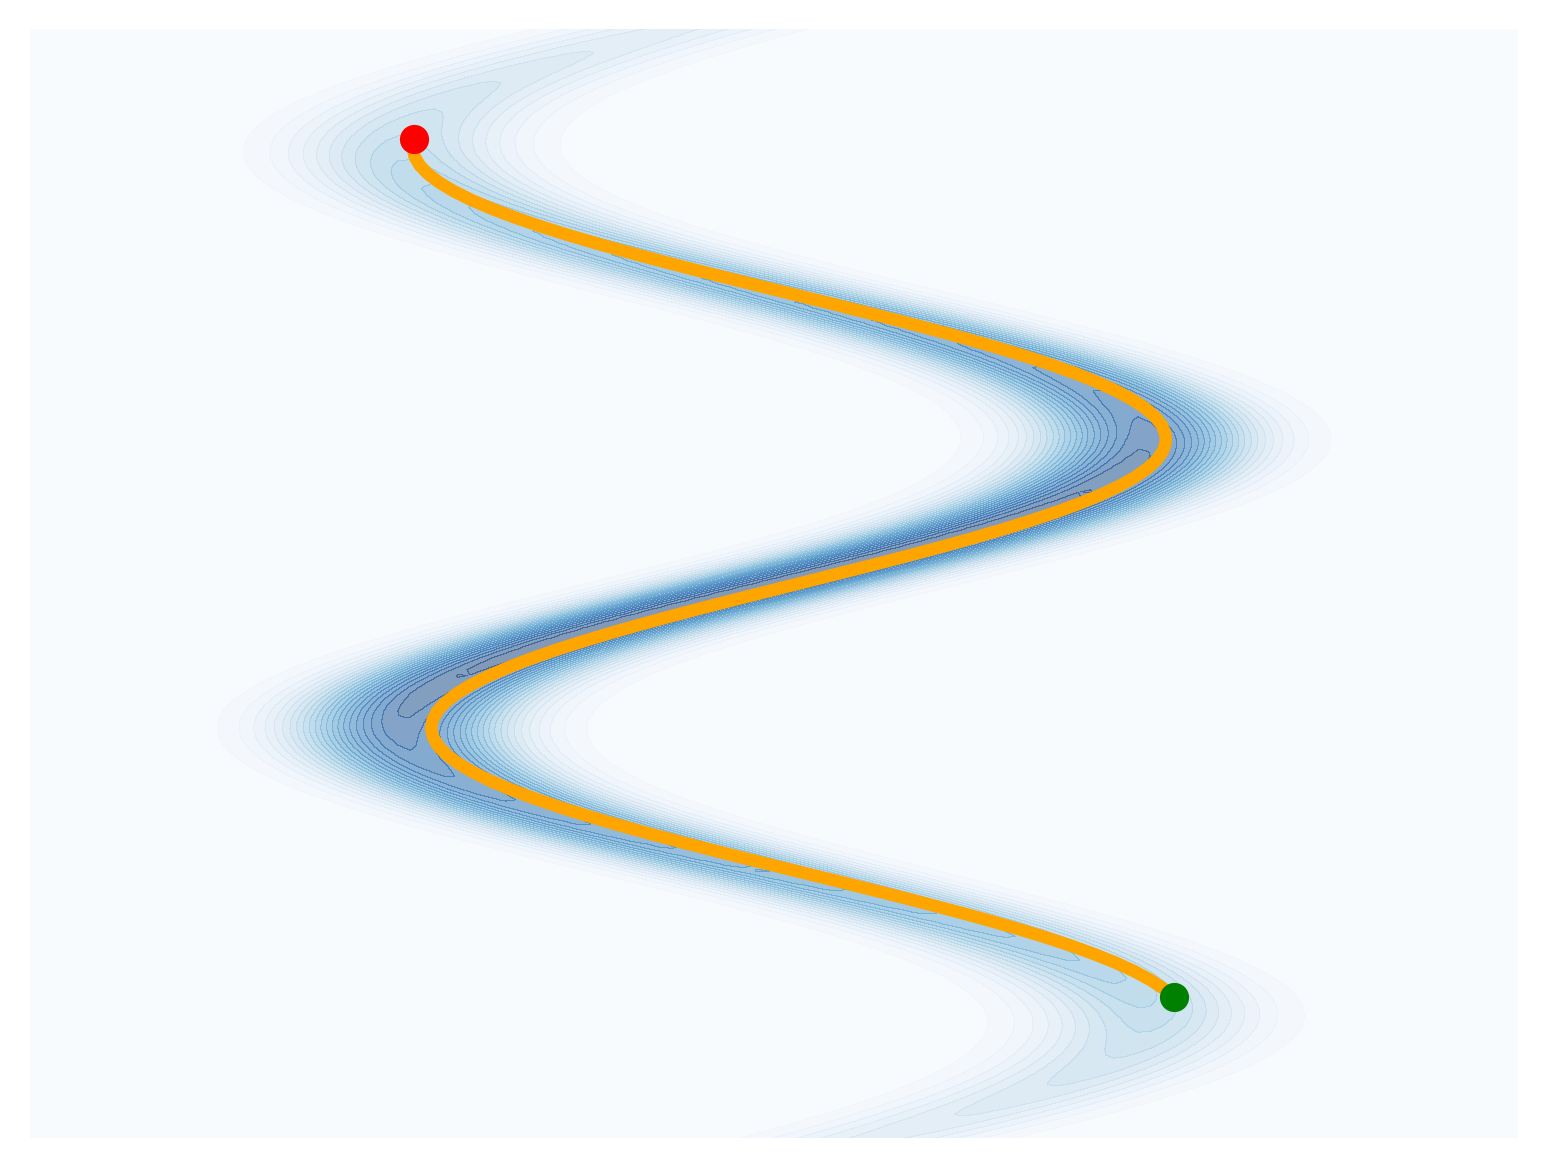
\includegraphics[width=\textwidth]{chapter5/results/visualisations/geodesics/gt.png}
            \caption{Ground Truth}
        \end{subfigure}
        \begin{subfigure}[b]{0.18\textwidth}
            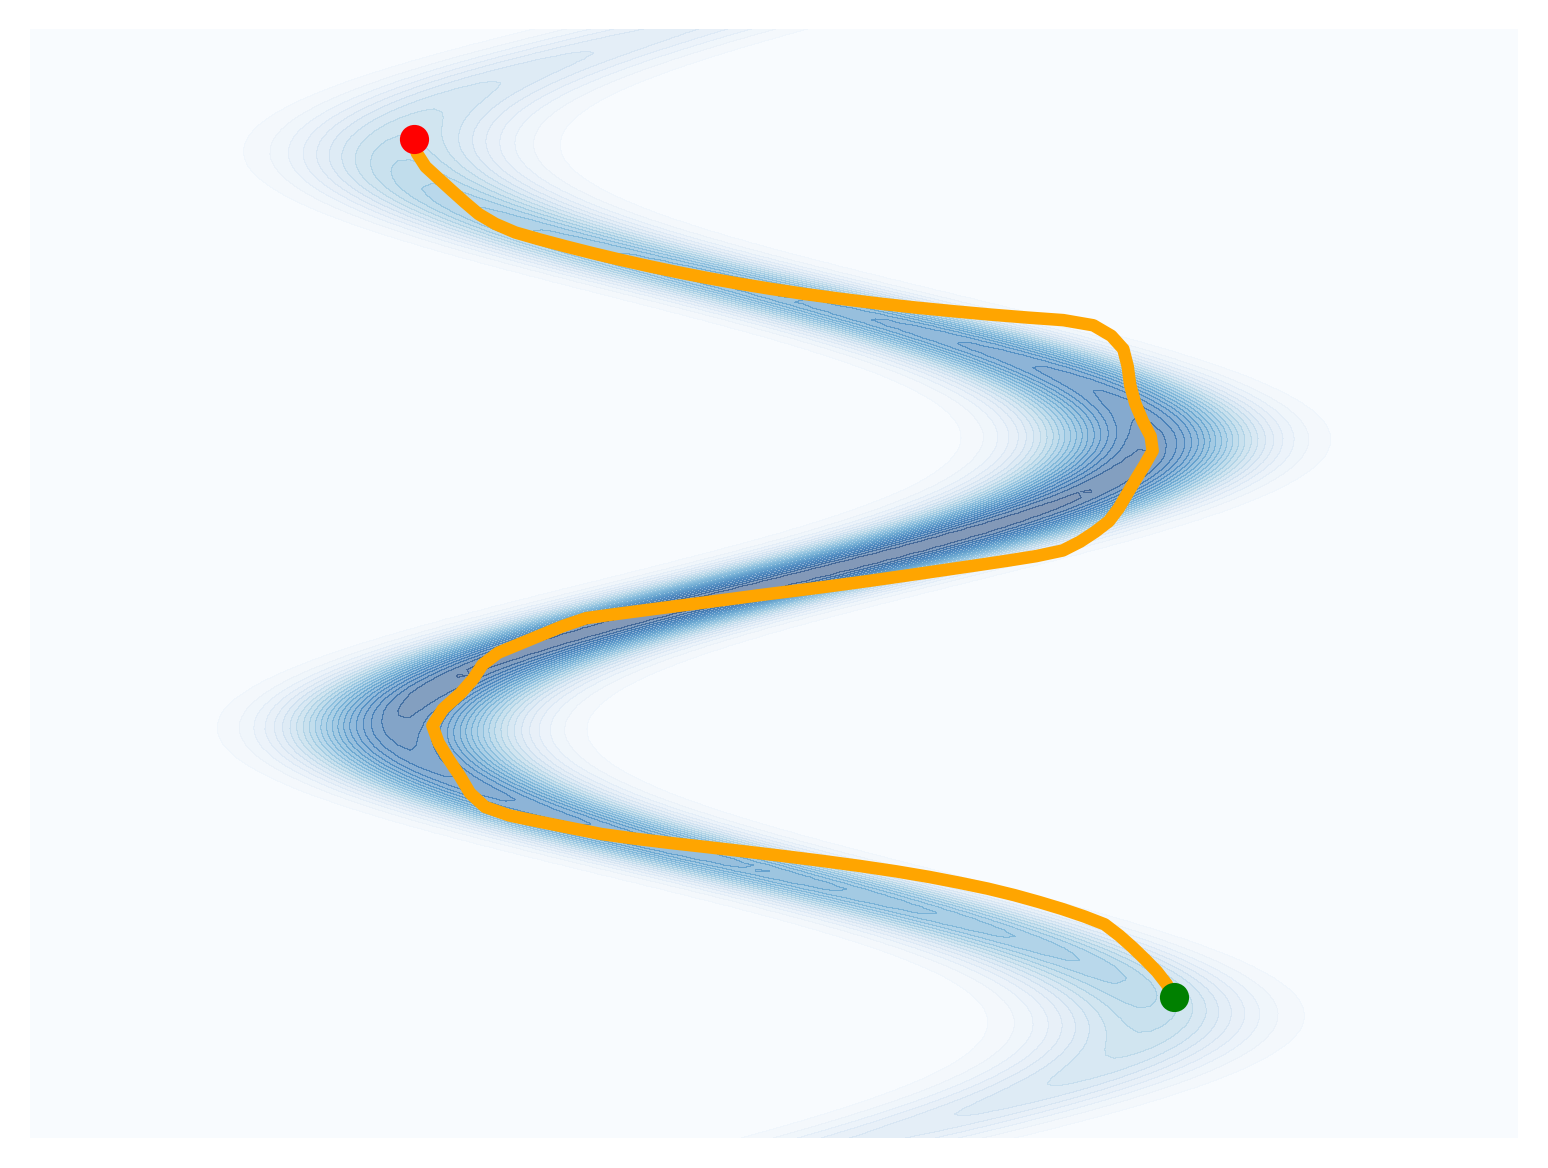
\includegraphics[width=\textwidth]{chapter5/results/visualisations/geodesics/ours.png}
            \caption{Our Method}
        \end{subfigure}
        \begin{subfigure}[b]{0.18\textwidth}
            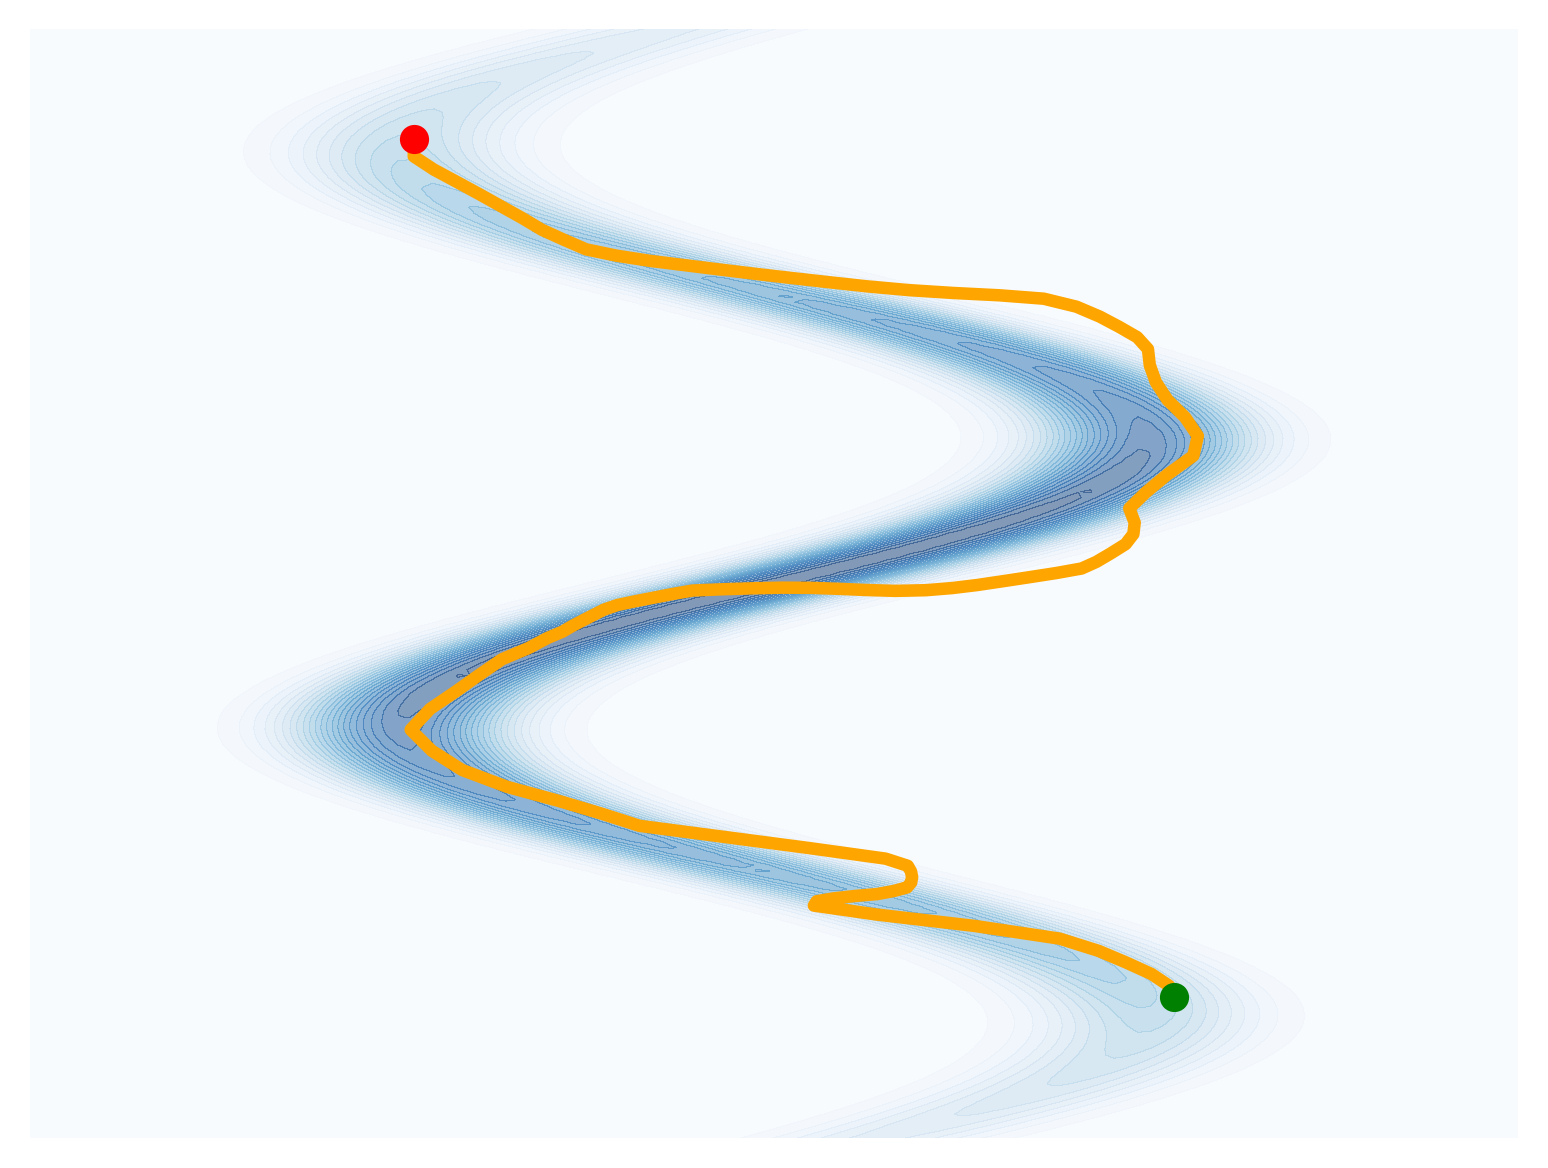
\includegraphics[width=\textwidth]{chapter5/results/visualisations/geodesics/standard_normal.png}
            \caption{Standard NF}
        \end{subfigure}
        \begin{subfigure}[b]{0.18\textwidth}
            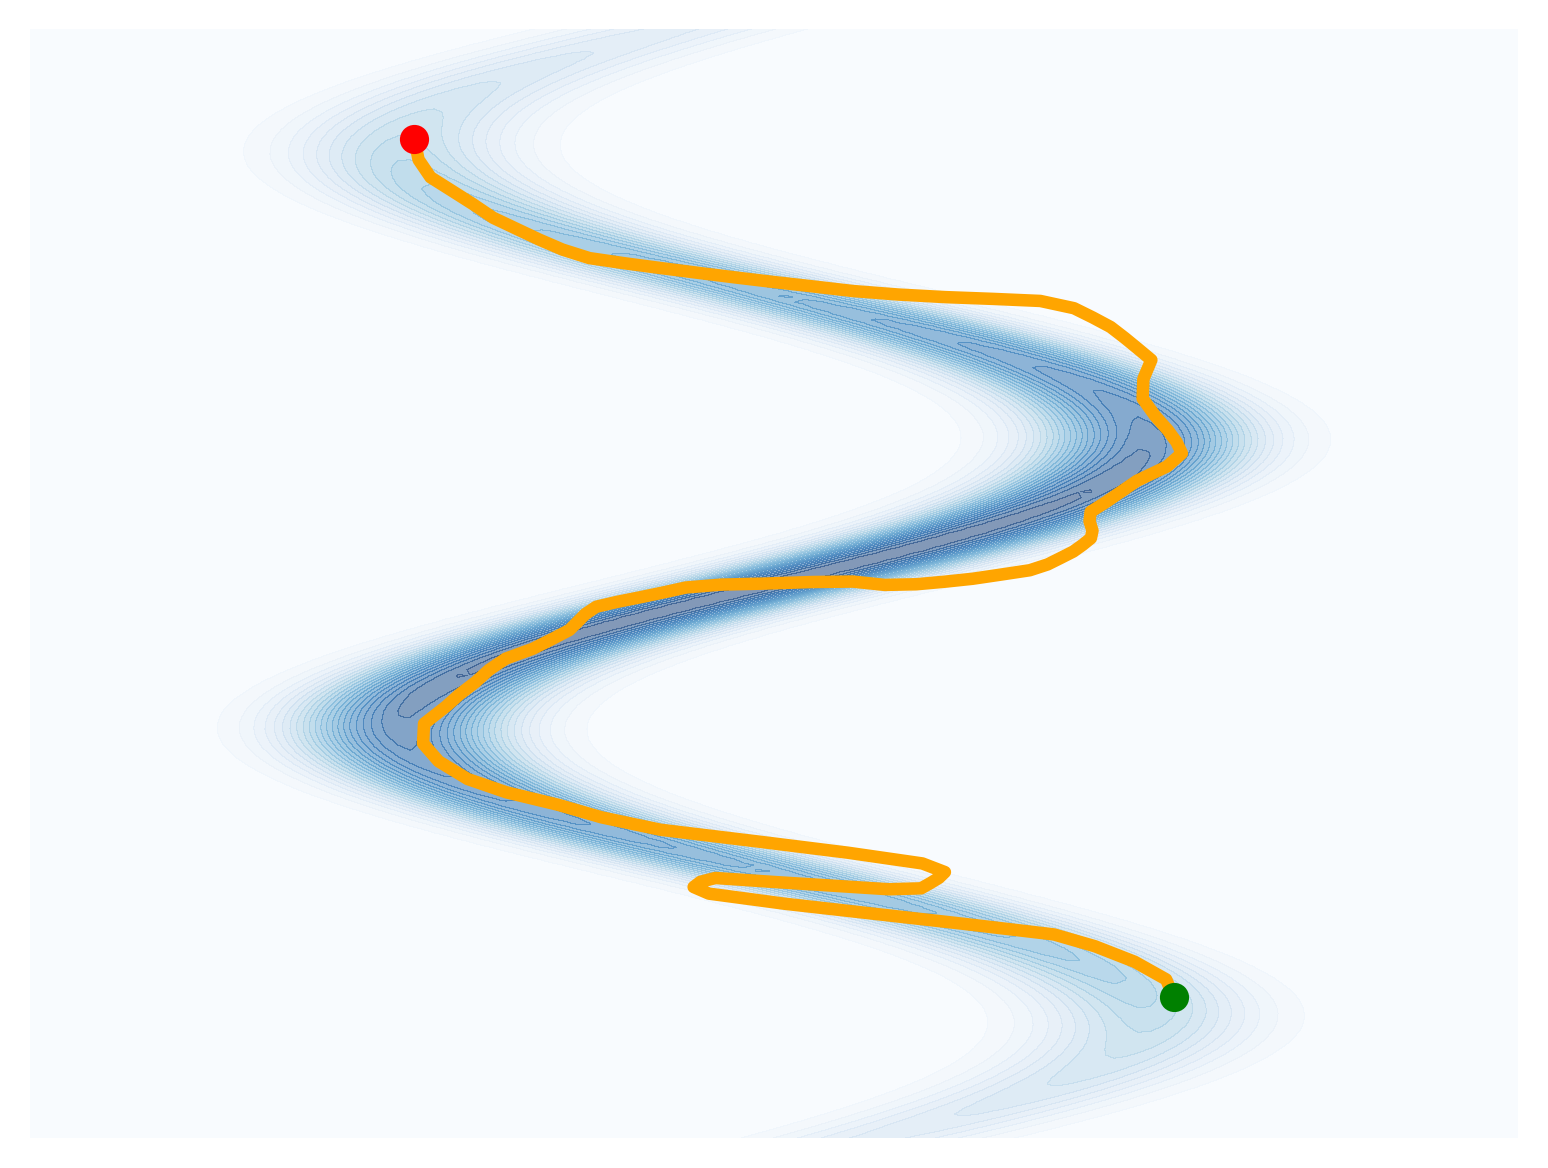
\includegraphics[width=\textwidth]{chapter5/results/visualisations/geodesics/standard_normal_anisotropic.png}
            \caption{Anisotropic NF}
        \end{subfigure}
        \begin{subfigure}[b]{0.18\textwidth}
            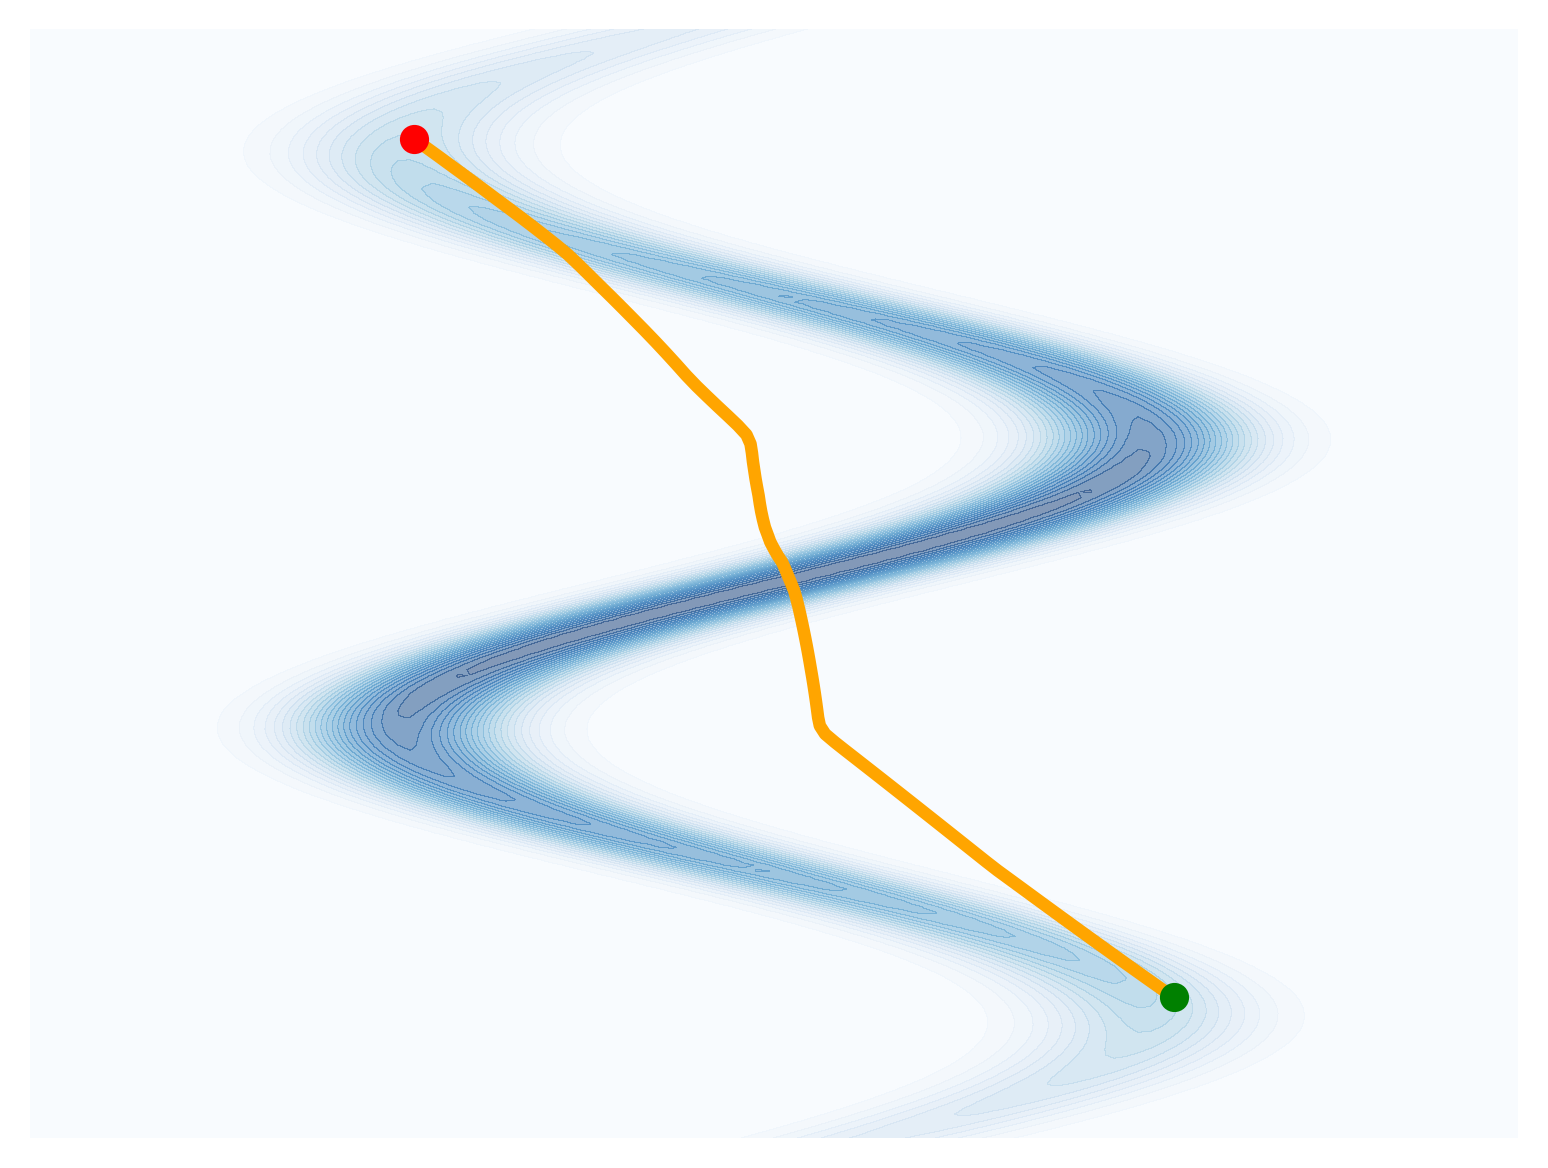
\includegraphics[width=\textwidth]{chapter5/results/visualisations/geodesics/isometricNF.png}
            \caption{Isometric NF}
        \end{subfigure}
        \caption{Comparison of geodesics computed using different methods on the river dataset. The geodesics generated by the proposed method have least artifacts, which is in line with our expectations from Table~\ref{tab:geodesic-variation-errors}.}
        \label{fig:geodesics_comparison}
    \end{figure}

\subsection{Riemannian autoencoder}
    \label{sec:RAE-experiments}
    To evaluate the capacity of our method to learn a Riemannian autoencoder, we conducted experiments on two synthetic datasets across various combinations of intrinsic dimension $\dimInd'$ and ambient dimension $\dimInd$:
    
    \begin{itemize}
        \item \textit{Hemisphere}($\dimInd'$, $\dimInd$): Samples are drawn from the upper hemisphere of a $\dimInd'$-dimensional unit sphere and embedded in an $\dimInd$-dimensional ambient space via a random isometric mapping.
        \item \textit{Sinusoid}($\dimInd'$, $\dimInd$): This dataset is generated by applying sinusoidal transformations to $\dimInd'$-dimensional latent variables, resulting in a complex, nonlinear manifold embedded in $\dimInd$ dimensions.
    \end{itemize}
    
    \noindent For a detailed description of these datasets, refer to \ref{app:rae_datasets}.

    \subsubsection{1D and 2D manifolds}
    In \ref{fig:learned_charts} and \ref{fig:learned_charts_for_Sinusoid_1_100}, we present the data manifold approximations by our Riemannian autoencoder for four low-dimensional manifolds.: Hemisphere(2,3), Sinusoid(1,3), Sinusoid(2,3) and Sinusoid(1,100). In \ref{app:data_manifold_approximation}, we detail the process used to create the data manifold approximations for these experiments. In our experiments, we set \( \epsilon = 0.01 \), which resulted in \( d_{\epsilon} = \dimInd' \) for all cases, accurately capturing the intrinsic dimension of each manifold and producing accurate global charts.

    \begin{figure}[htb]
        \centering
    
        % First row: Projections of RAE for three datasets
        \begin{subfigure}[b]{0.32\textwidth}
            \centering
            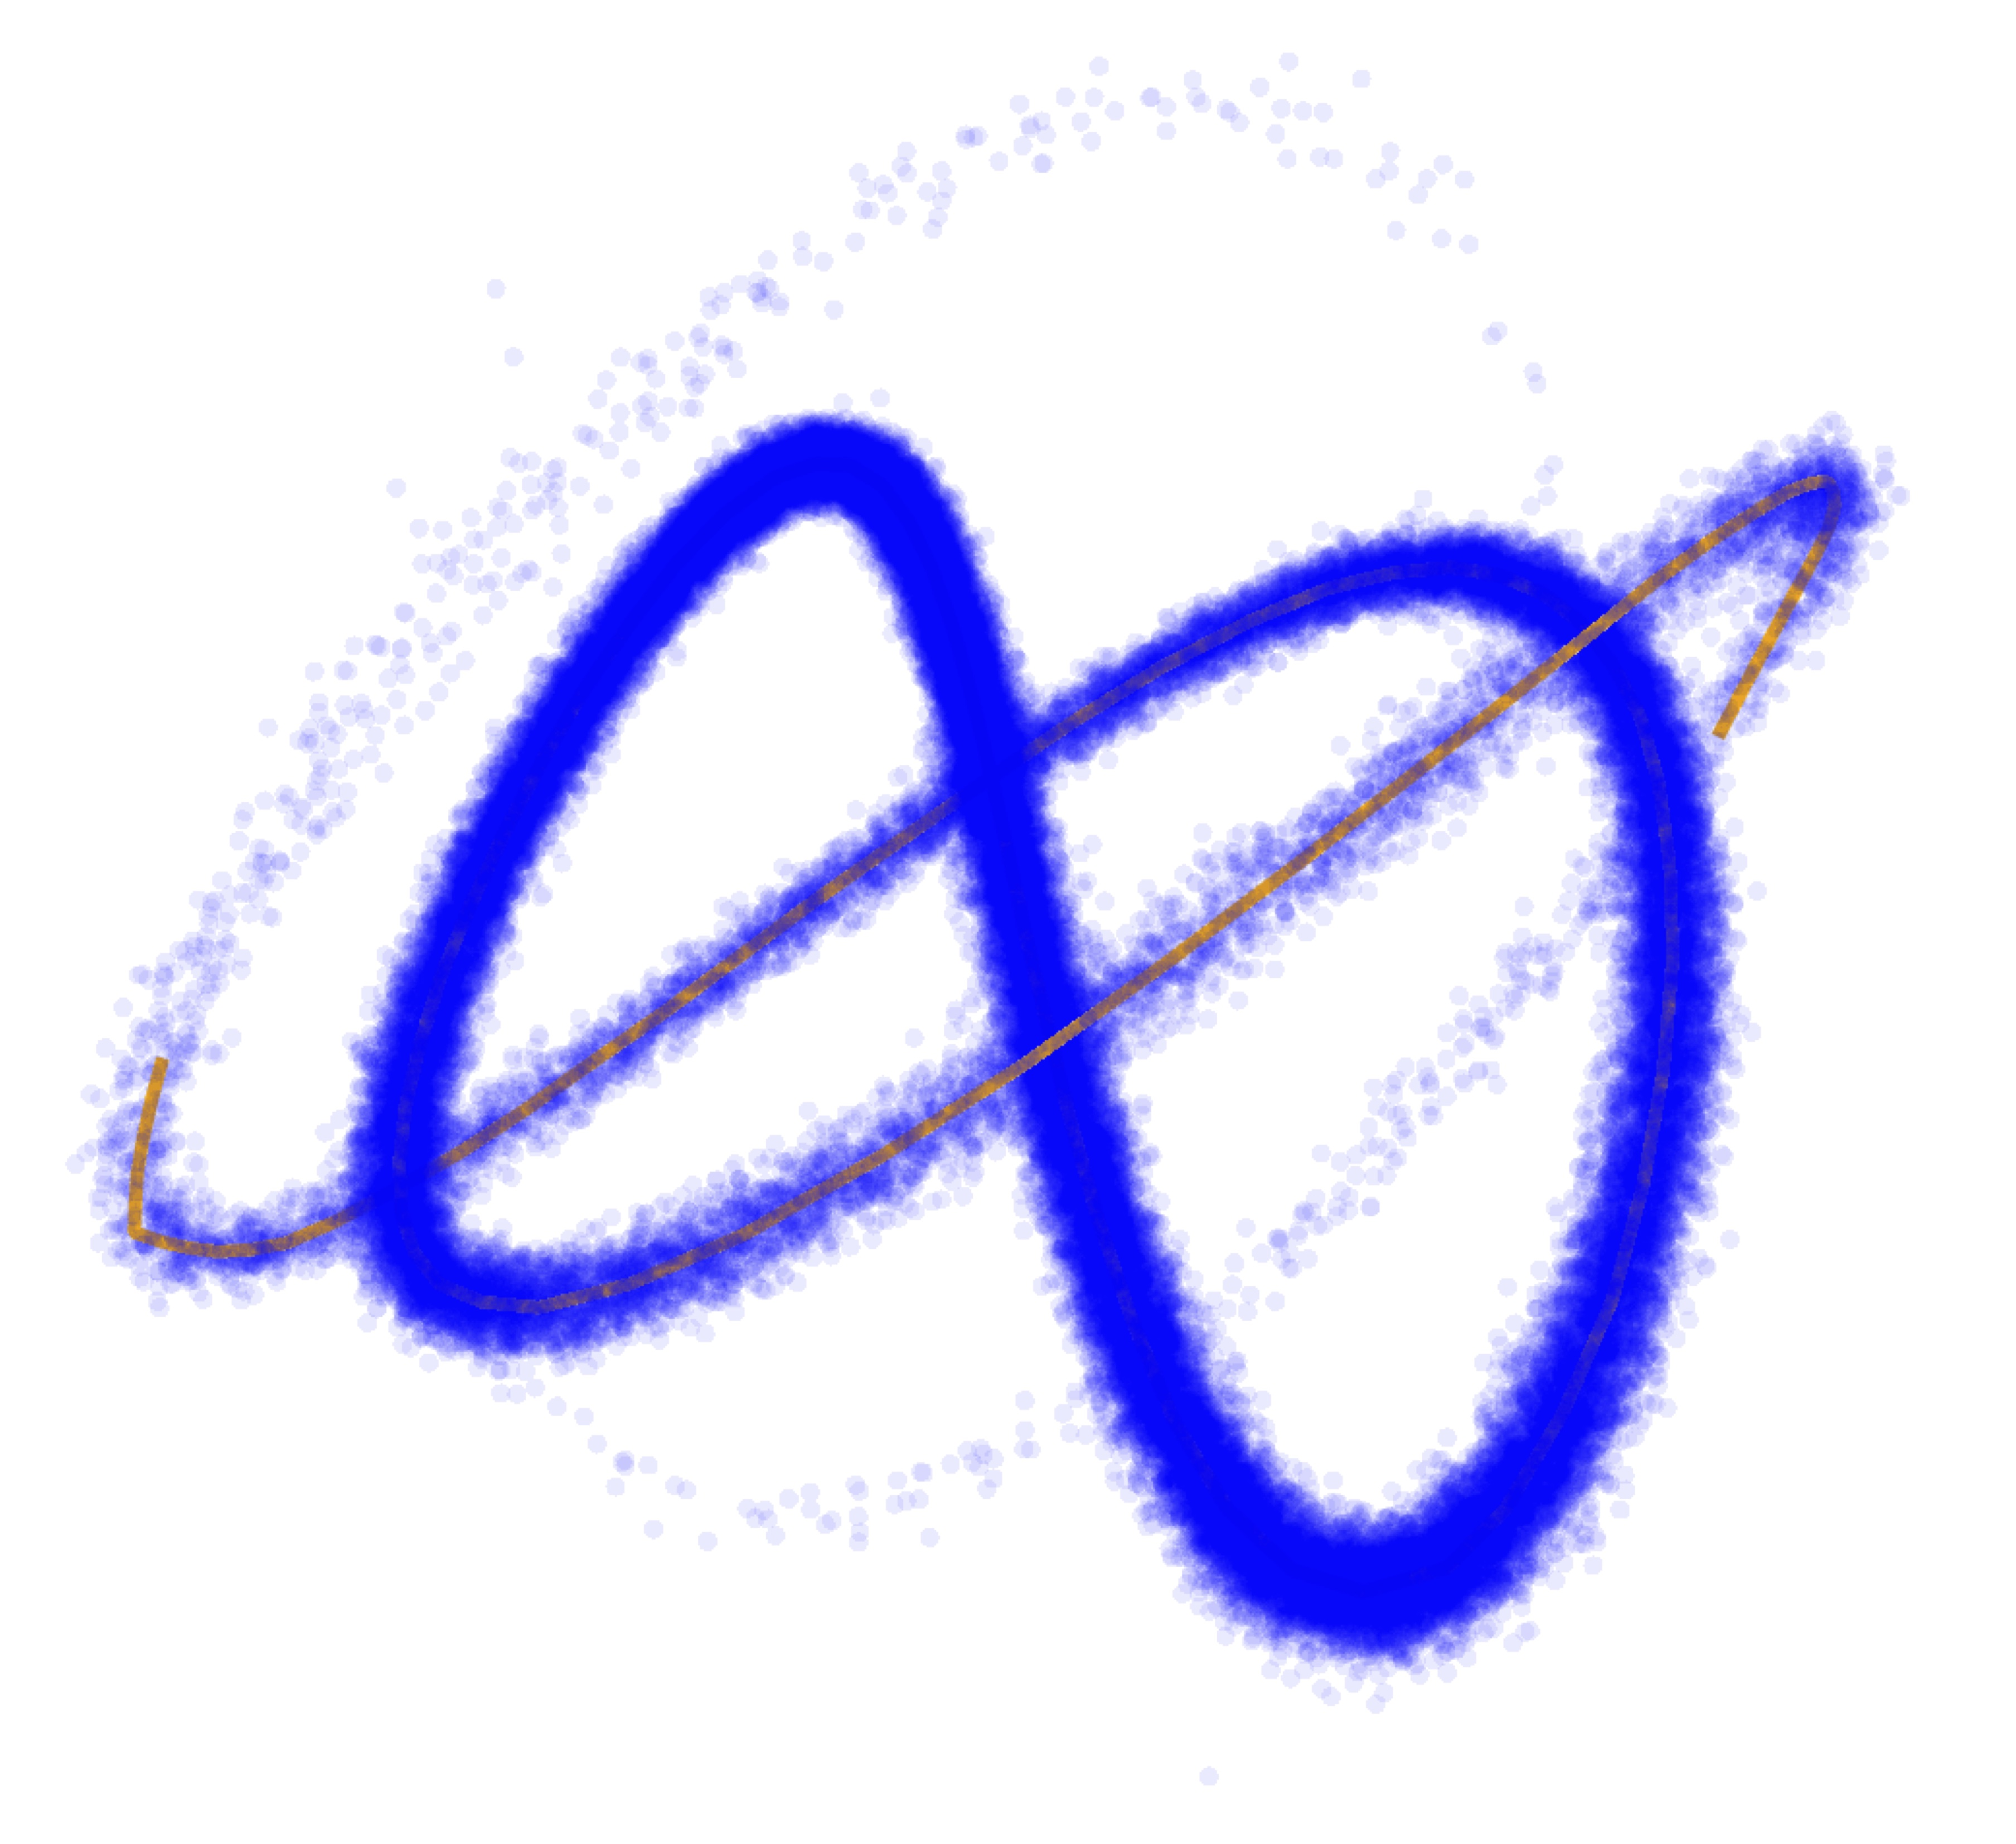
\includegraphics[width=\textwidth]{chapter5/results/visualisations/RAE/projections/sinusoid_1_100/more_transparent/5_59_92.jpg}
            \caption{Dims (5, 59, 92)}
        \end{subfigure}
        \hfill
        \begin{subfigure}[b]{0.32\textwidth}
            \centering
            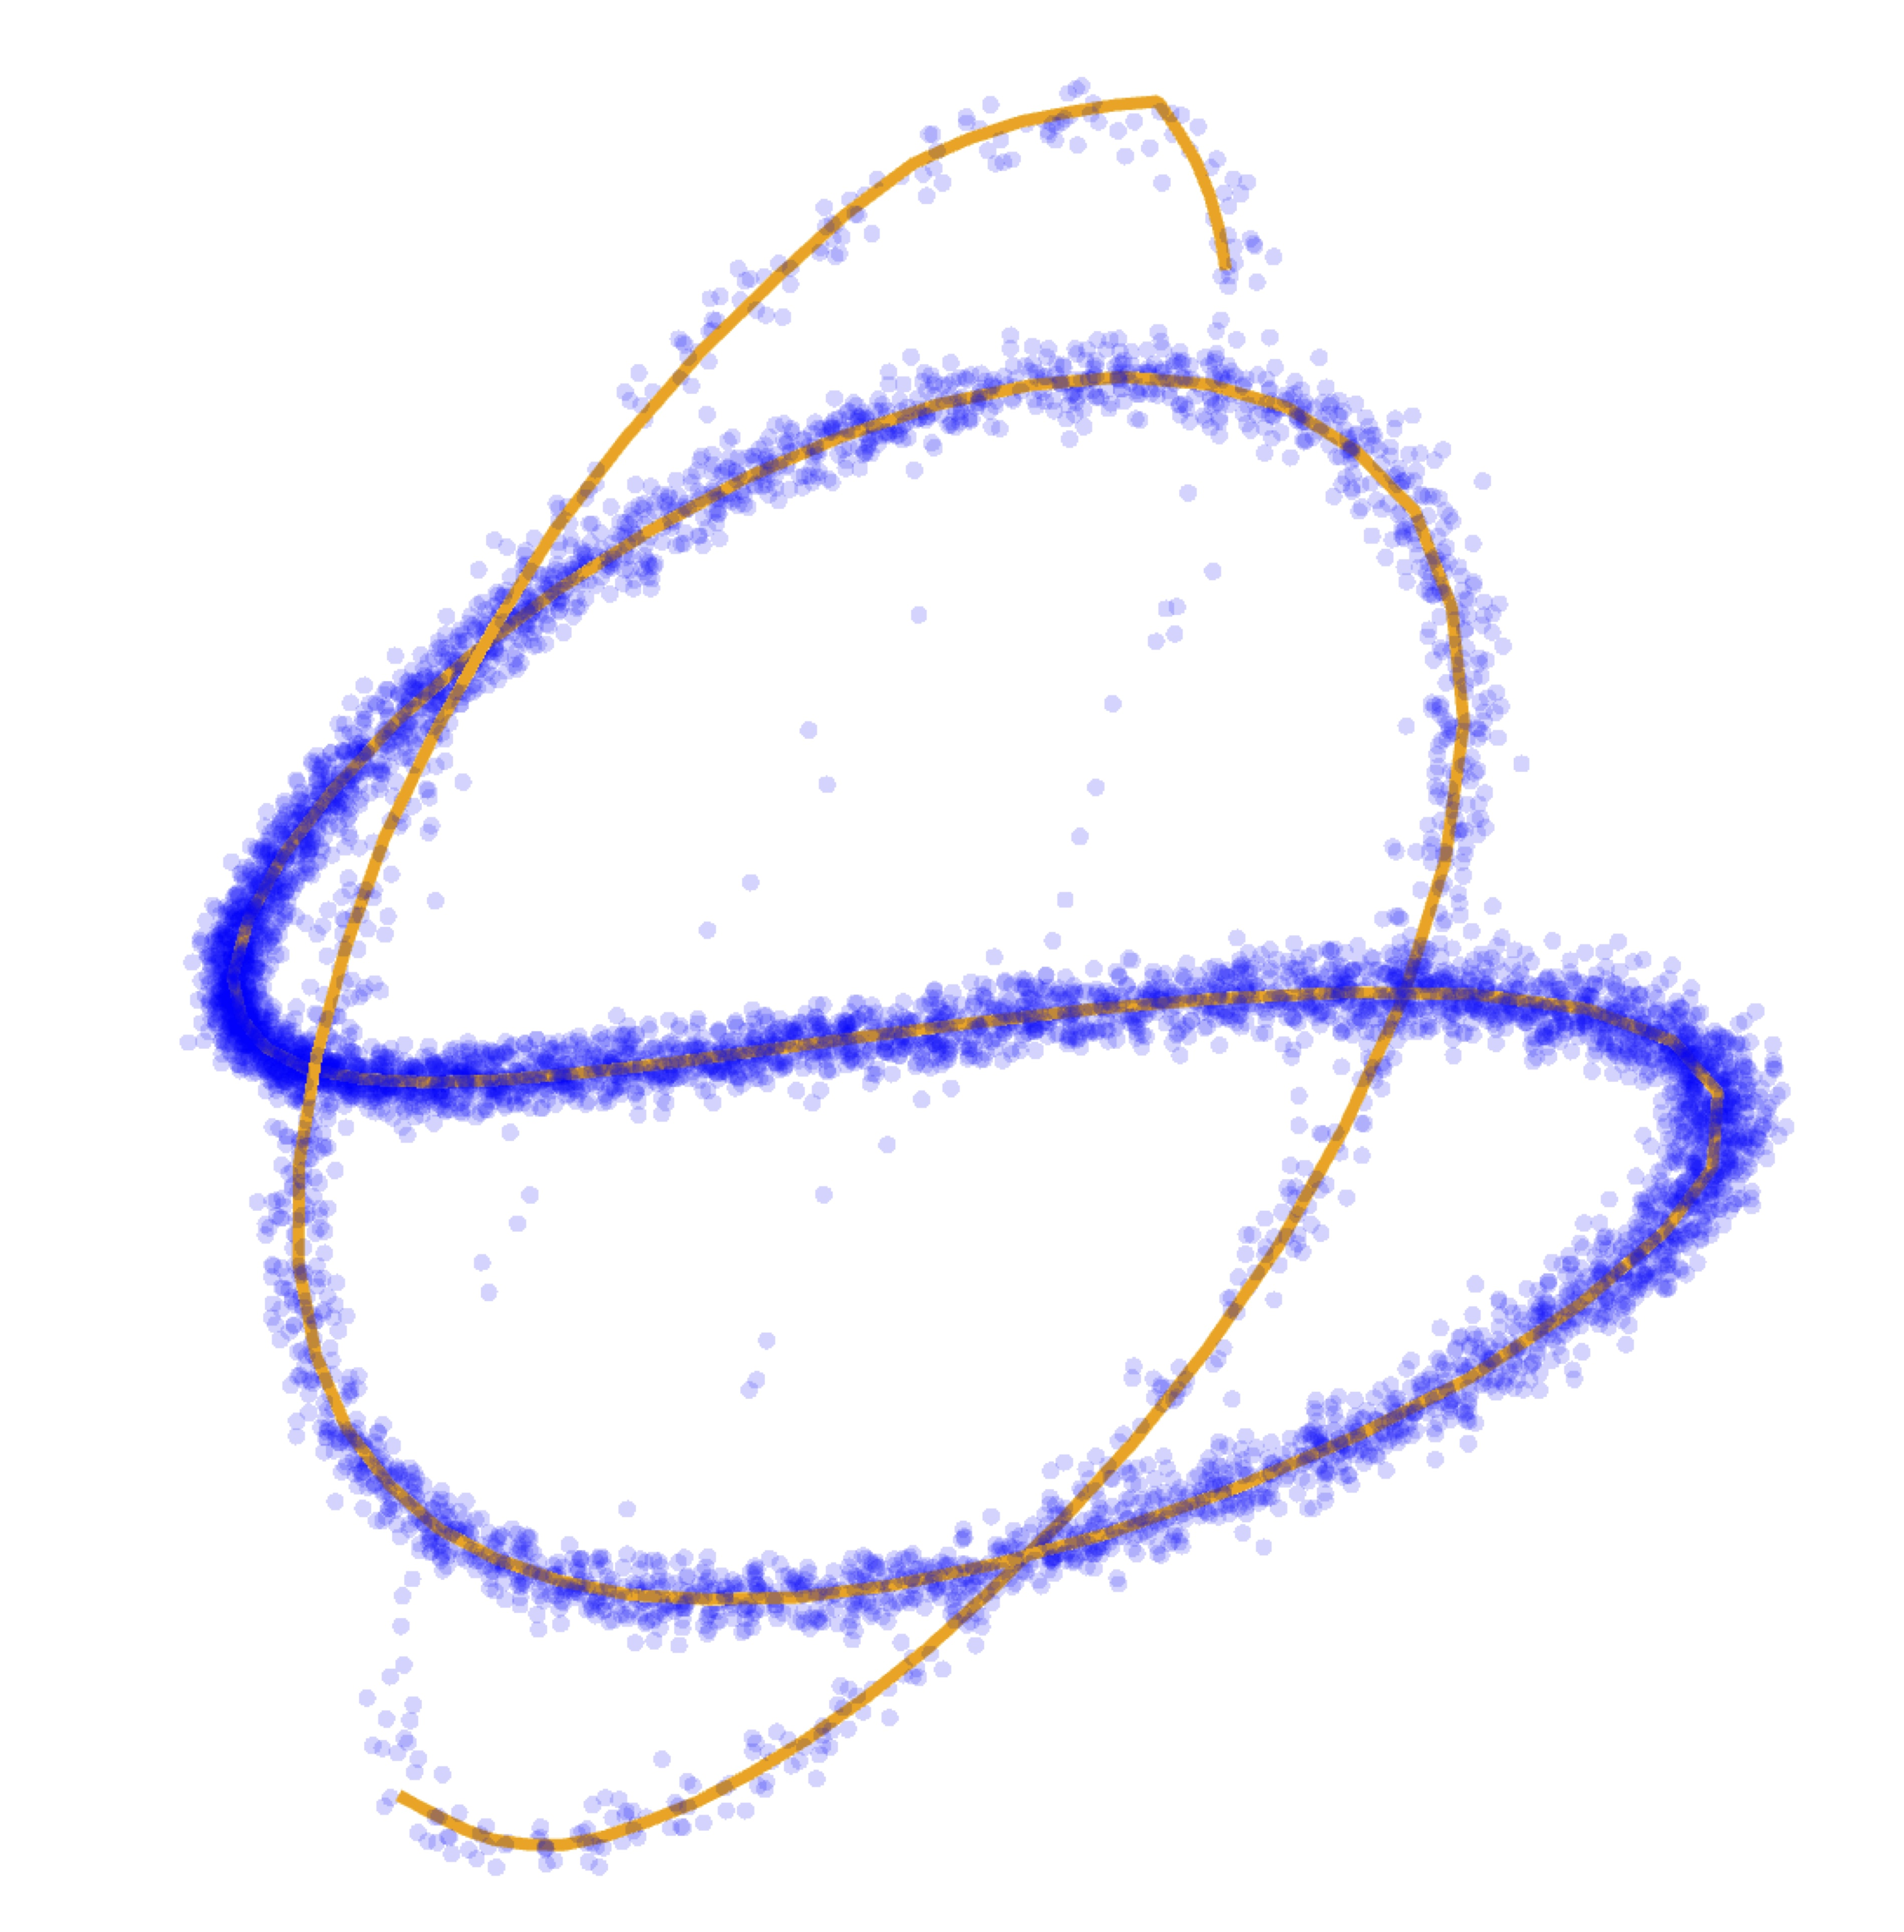
\includegraphics[width=\textwidth]{chapter5/results/visualisations/RAE/projections/sinusoid_1_100/more_transparent/31_55_66.jpg}
            \caption{Dims (31, 55, 66)}
        \end{subfigure}
        \hfill
        \begin{subfigure}[b]{0.32\textwidth}
            \centering
            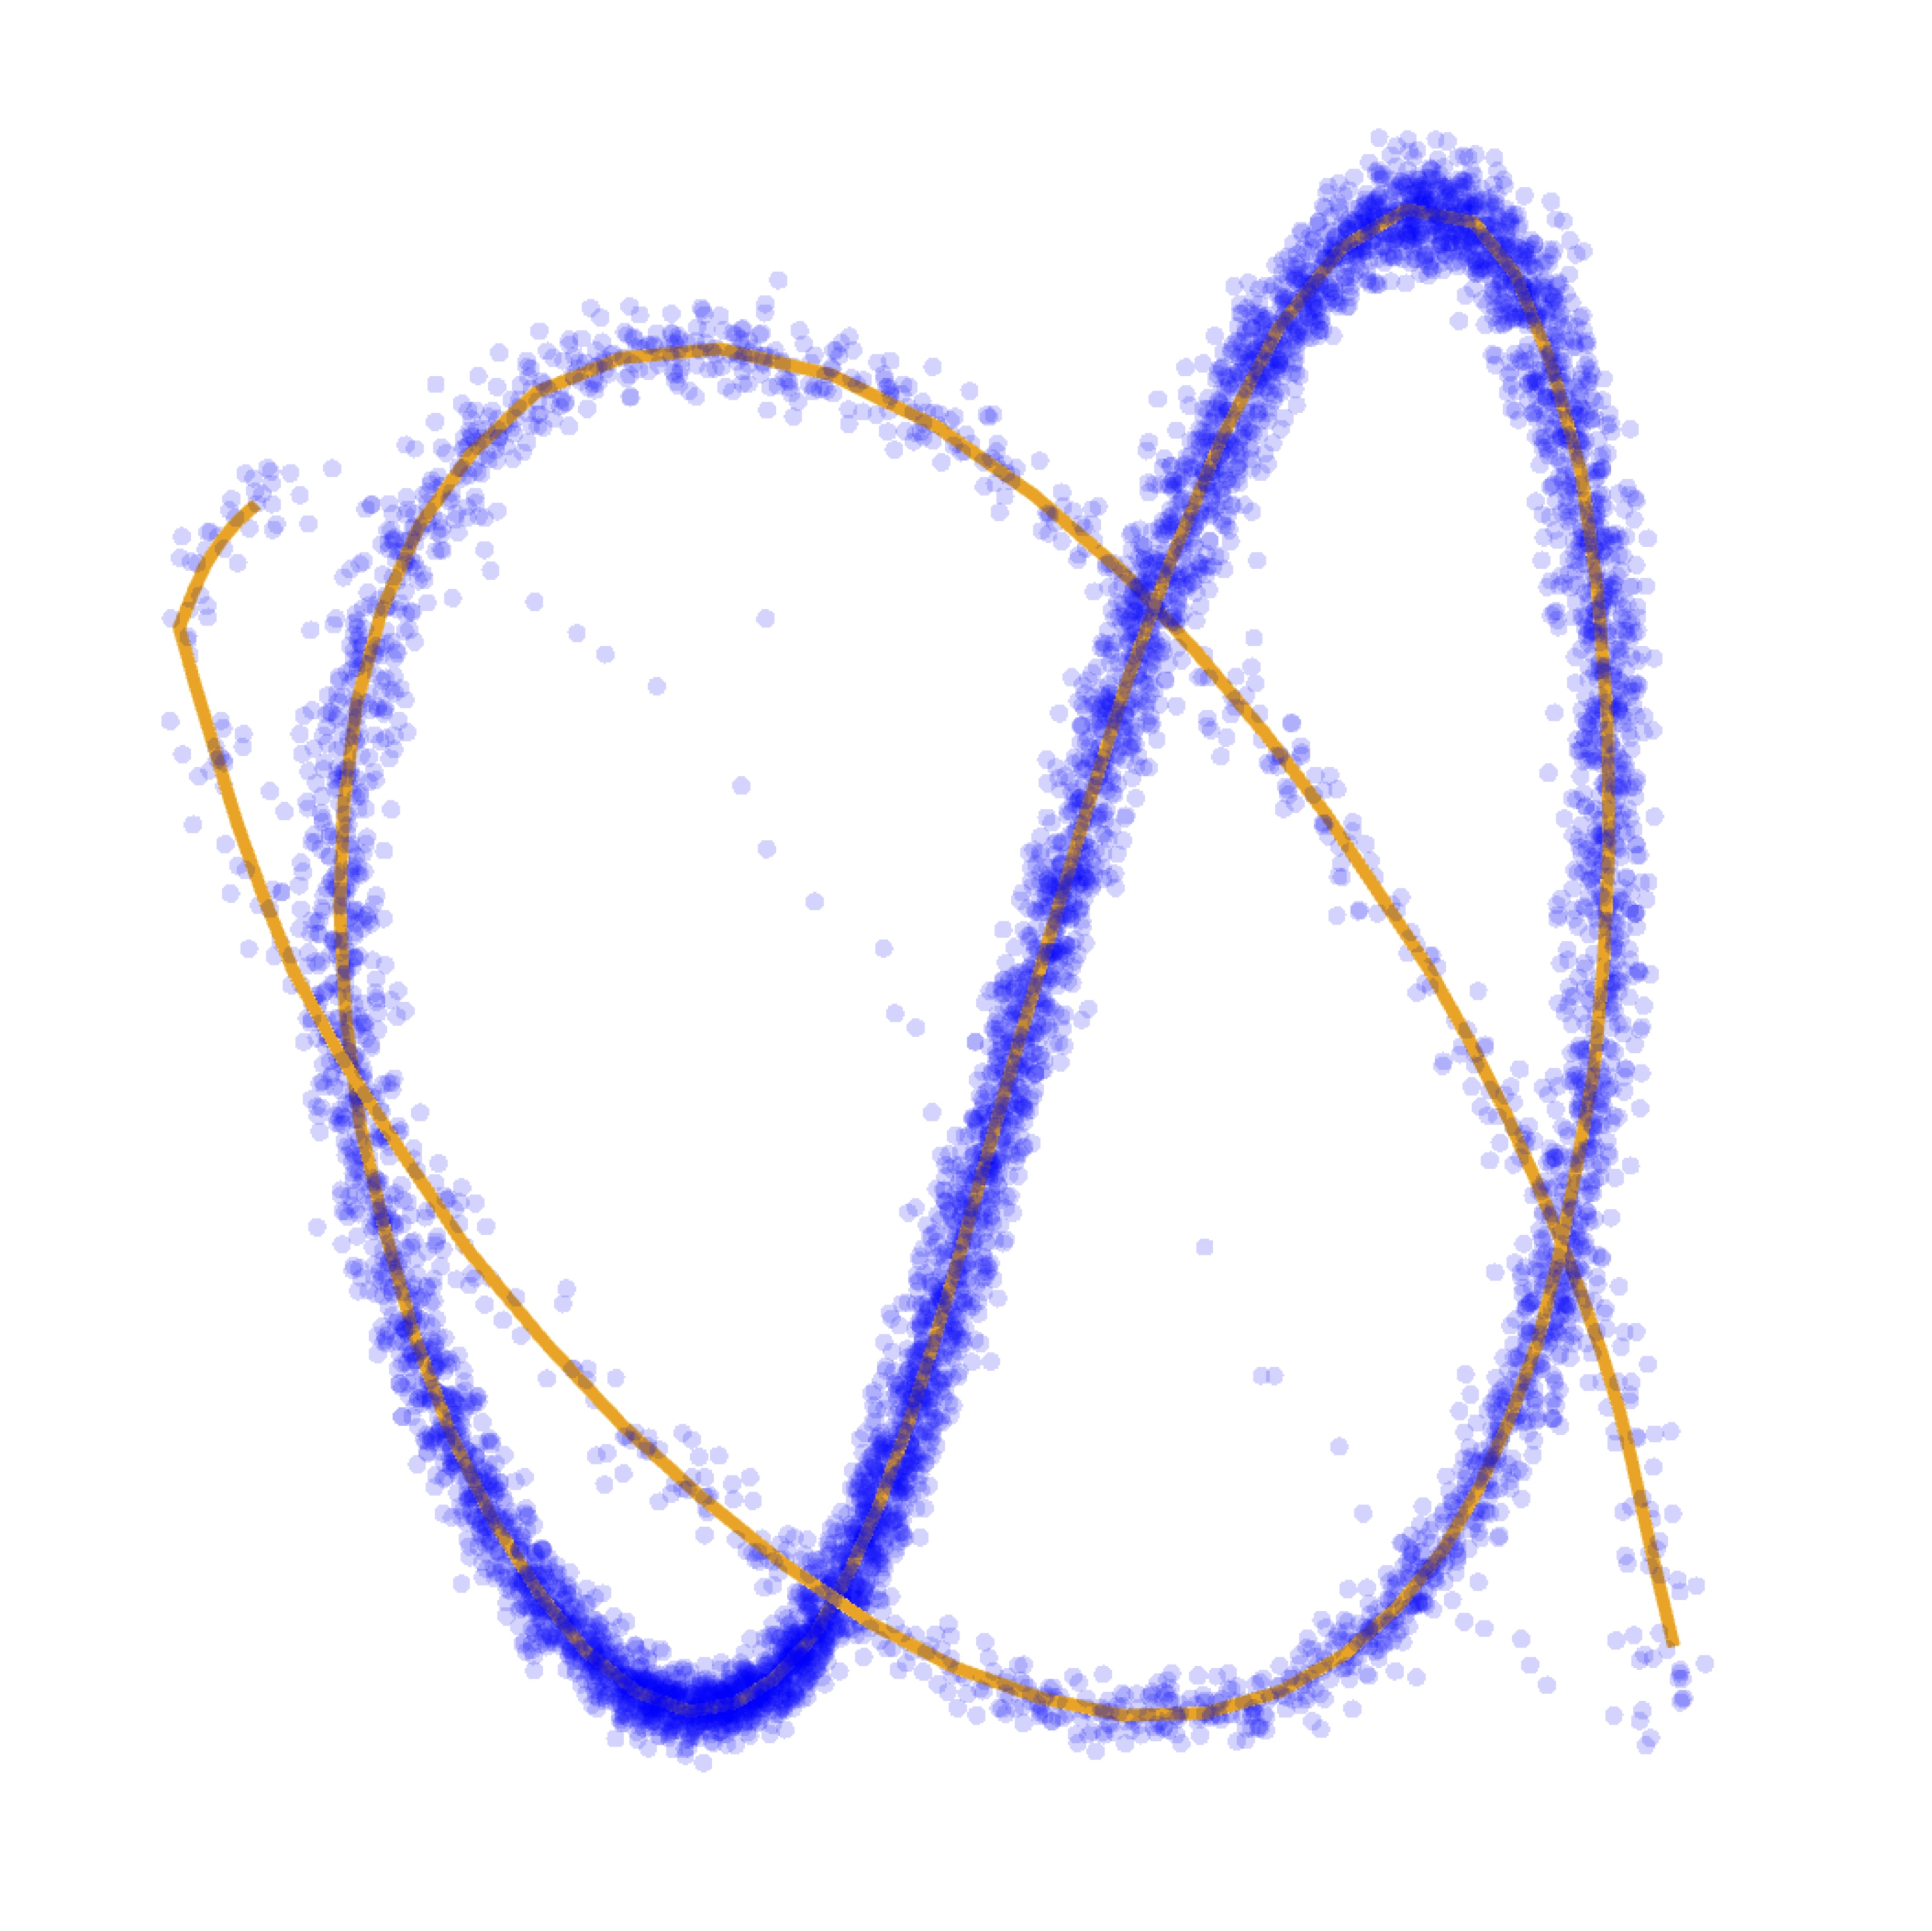
\includegraphics[width=\textwidth]{chapter5/results/visualisations/RAE/projections/sinusoid_1_100/more_transparent/64_72_90.jpg}
            \caption{Dims (64, 72, 90)}
        \end{subfigure}
    
        \caption{
            Approximate data manifold learned by the Riemannian autoencoder for the Sinusoid(1, 100) dataset. The orange curves depict the manifold learned by the model, while the blue points show the training data. We visualize three different combinations of the ambient dimensions. %to illustrate how the 1-dimensional manifold is embedded in the higher-dimensional ambient space.
        }
        \label{fig:learned_charts_for_Sinusoid_1_100}
    \end{figure}


    \subsubsection{Higher-dimensional manifolds}




    To evaluate the scalability of our method to higher-dimensional manifolds, we conducted additional experiments on the Hemisphere(5,20) and Sinusoid(5,20) datasets. 
    
    Our theory suggests that the learned variances indicate the importance of each latent dimension: higher variances signal more important dimensions for reconstructing the manifold, while dimensions with vanishing variances are considered insignificant and are disregarded when constructing the Riemannian autoencoder. To test the model's ability to correctly identify important and unimportant latent dimensions, we report the average $\ell^2$ reconstruction error for each dataset as a function of the number of latent dimensions used. In the reconstruction error plots (see \ref{fig:hemisphere_reconstruction_errors},\ref{fig:sinusoid_reconstruction_errors}), we report three variance-based orders for adding latent dimensions: decreasing variance order (blue line), increasing variance order (green line), and random order (red line).
    
    For the Hemisphere(5,20) dataset, the model identified five non-vanishing variances (see \ref{fig:hemisphere_variances}), perfectly capturing the intrinsic dimension of the manifold. This is reflected in the blue curve in \ref{fig:hemisphere_reconstruction_errors}, where the first five latent dimensions, corresponding to the largest variances, are sufficient to reduce the reconstruction error almost to zero. In contrast, the green curve illustrates that the remaining ambient dimensions do not encode useful information about the manifold. The red curve demonstrates improvement only when an important latent dimension is included.
    
    For the more challenging Sinusoid(5,20) dataset, our method still performs very well, though not as perfectly as for the Hemisphere dataset. The first six most important latent dimensions explain approximately $97\%$ of the variance, increasing to over $99\%$ with the seventh dimension (see \ref{fig:sinusoid_variances}). This is reflected in the blue curve in \ref{fig:sinusoid_reconstruction_errors}, where the first six latent dimensions reduce the reconstruction error to near zero, and the addition of the seventh dimension brings the error effectively to zero. The slight discrepancy between our results and the ground truth likely arises from increased optimization difficulty, as the normalizing flow must learn a more intricate distribution while maintaining approximate isometry. We believe that with deeper architectures and more careful tuning of the optimization loss, the model will converge to the correct intrinsic dimensionality of five. Currently, it predicts six dimensions at a threshold of $\epsilon = 0.05$ and seven at $\epsilon = 0.01$, slightly overestimating due to the manifold's complexity.
    
    \begin{figure}[t!]
        \vspace{-0.5cm}
            \centering
            % Title for Hemisphere
            \textbf{Hemisphere (5,20)} \par\medskip
            
            % First row: Hemisphere plots
            \begin{subfigure}[b]{0.443\textwidth}
                \centering
                \includegraphics[width=\textwidth]{chapter5/results/visualisations/RAE/reconstruction/hemisphere_5_20/diagonal_values_normal_scale.png}
                \caption{Learned variances in decreasing order.}
                \label{fig:hemisphere_variances}
            \end{subfigure}
            \hfill
            \begin{subfigure}[b]{0.546\textwidth}
                \centering
                \includegraphics[width=\textwidth]{chapter5/results/visualisations/RAE/reconstruction/hemisphere_5_20/reconstruction_error_plot_normal_scale.png}
                \caption{Reconstruction error for three latent orders.}
                \label{fig:hemisphere_reconstruction_errors}
            \end{subfigure}
            
            \vspace{1.5em} % Add some space between the rows
            
            % Title for Sinusoid
            \textbf{Sinusoid (5,20)} \par\medskip
            
            % Second row: Sinusoid plots
            \begin{subfigure}[b]{0.440\textwidth}
                \centering
                \includegraphics[width=\textwidth]{chapter5/results/visualisations/RAE/reconstruction/sinusoid_5_20/diagonal_values_normal_scale.png}
                \caption{Learned variances in decreasing order.}
                \label{fig:sinusoid_variances}
            \end{subfigure}
            \hfill
            \begin{subfigure}[b]{0.549\textwidth}
                \centering
                \includegraphics[width=\textwidth]{chapter5/results/visualisations/RAE/reconstruction/sinusoid_5_20/reconstruction_error_plot_normal_scale.png}
                \caption{Reconstruction error for three latent orders.}
                \label{fig:sinusoid_reconstruction_errors}
            \end{subfigure}
        
            % Main caption for the entire figure
            \caption{Learned variances and reconstruction errors for the Hemisphere(5,20) and Sinusoid(5,20) datasets. The plots in the left column show the learned variances in decreasing order for each dataset, while the right column illustrates the average $\ell^2$ reconstruction error as a function of the number of latent dimensions used. The reconstruction errors are evaluated for three variance-based orders of the latent dimensions: the \textbf{blue line} (circular markers) represents adding dimensions in decreasing order of variance, the \textbf{green line} (square markers) for increasing variance, and the \textbf{red line} (diamond markers) for a random order.\vspace{-2em}
        }
        
            \label{fig:combined_plot}
        \end{figure}

        \section{Conclusions}
\label{sec:conclusions}

In this work we have taken a first step towards a practical Riemannian geometry framework for generative modelling, striking a balance between scalability of training a data-driven Riemannian structure and of evaluating its corresponding manifold mappings. We have considered a family of unimodal probability densities whose negative log-likelihoods are compositions of strongly convex functions and diffeomorphisms, and sought to learn them. We have shown that once these unimodal densities have been learned, the proposed score-based pullback geometry gives us closed-form geodesics that pass through the data probability density and a Riemannian autoencoder with error bounds that can be used to estimate the dimension of the %correct (approximate) 
data manifold. Finally, to learn the distribution we have proposed an adaptation to normalizing flow training. Through numerical experiments, we have shown that these modifications are crucial for extracting geometric information, and that our framework not only generates high-quality geodesics across the data support, but also accurately estimates the intrinsic dimension of the approximate data manifold while constructing a global chart, even in high-dimensional ambient spaces. Current challenges of the method lie in balancing the expressivity of the network architecture, e.g., through additional layers or more expressive architectures, and satisfying approximate $\ell^2$-isometry on the data support. For future work we aim to overcome these challenges, extending the method to multimodal distributions, while making it scalable for higher-dimensional data sets.
